% ---- ETD Document Class and Useful Packages ---- %
\documentclass{ucetd}
\usepackage{subfigure,epsfig,amsfonts}
\usepackage{natbib}
\usepackage{amsmath}
\usepackage{amssymb}
\usepackage{amsthm}
\usepackage[utf8]{inputenc}
\usepackage{listings}
\usepackage{xcolor}

\usepackage[english]{babel}
\usepackage[T1]{fontenc}



\definecolor{codegreen}{rgb}{0,0.6,0}
\definecolor{codegray}{rgb}{0.5,0.5,0.5}
\definecolor{codepurple}{rgb}{0.58,0,0.82}
\definecolor{backcolour}{rgb}{0.95,0.95,0.92}

% for ipython formatting
\definecolor{maroon}{cmyk}{0, 0.87, 0.68, 0.32}
\definecolor{halfgray}{gray}{0.55}
\definecolor{ipython_frame}{RGB}{207, 207, 207}
\definecolor{ipython_bg}{RGB}{247, 247, 247}
\definecolor{ipython_red}{RGB}{186, 33, 33}
\definecolor{ipython_green}{RGB}{0, 128, 0}
\definecolor{ipython_cyan}{RGB}{64, 128, 128}
\definecolor{ipython_purple}{RGB}{170, 34, 255}

% for R formatting
\definecolor{dkgreen}{rgb}{0,0.6,0}
\definecolor{gray}{rgb}{0.5,0.5,0.5}
\definecolor{mauve}{rgb}{0.58,0,0.82}

% generic code style
\lstdefinestyle{mystyle}{
    backgroundcolor=\color{backcolour},   
    commentstyle=\color{codegreen},
    keywordstyle=\color{magenta},
    numberstyle=\tiny\color{codegray},
    stringstyle=\color{codepurple},
    basicstyle=\ttfamily\footnotesize,
    breakatwhitespace=false,         
    breaklines=true,                 
    captionpos=b,                    
    keepspaces=true,                 
    numbers=left,                    
    numbersep=5pt,                  
    showspaces=false,                
    showstringspaces=false,
    showtabs=false,                  
    tabsize=2
}


\lstset{
    breaklines=true,
    %
    extendedchars=true,
    literate=
    {á}{{\'a}}1 {é}{{\'e}}1 {í}{{\'i}}1 {ó}{{\'o}}1 {ú}{{\'u}}1
    {Á}{{\'A}}1 {É}{{\'E}}1 {Í}{{\'I}}1 {Ó}{{\'O}}1 {Ú}{{\'U}}1
    {à}{{\`a}}1 {è}{{\`e}}1 {ì}{{\`i}}1 {ò}{{\`o}}1 {ù}{{\`u}}1
    {À}{{\`A}}1 {È}{{\'E}}1 {Ì}{{\`I}}1 {Ò}{{\`O}}1 {Ù}{{\`U}}1
    {ä}{{\"a}}1 {ë}{{\"e}}1 {ï}{{\"i}}1 {ö}{{\"o}}1 {ü}{{\"u}}1
    {Ä}{{\"A}}1 {Ë}{{\"E}}1 {Ï}{{\"I}}1 {Ö}{{\"O}}1 {Ü}{{\"U}}1
    {â}{{\^a}}1 {ê}{{\^e}}1 {î}{{\^i}}1 {ô}{{\^o}}1 {û}{{\^u}}1
    {Â}{{\^A}}1 {Ê}{{\^E}}1 {Î}{{\^I}}1 {Ô}{{\^O}}1 {Û}{{\^U}}1
    {œ}{{\oe}}1 {Œ}{{\OE}}1 {æ}{{\ae}}1 {Æ}{{\AE}}1 {ß}{{\ss}}1
    {ç}{{\c c}}1 {Ç}{{\c C}}1 {ø}{{\o}}1 {å}{{\r a}}1 {Å}{{\r A}}1
    {€}{{\EUR}}1 {£}{{\pounds}}1
}

%%
%% Python definition (c) 1998 Michael Weber
%% Additional definitions (2013) Alexis Dimitriadis
%% modified by me (should not have empty lines)
%%

%% Very sexy ipython code formatting
\lstdefinelanguage{iPython}{
    morekeywords={access,and,break,class,continue,def,del,elif,else,except,exec,finally,for,from,global,if,import,in,is,lambda,not,or,pass,print,raise,return,try,while},%
    %
    % Built-ins
    morekeywords=[2]{abs,all,any,basestring,bin,bool,bytearray,callable,chr,classmethod,cmp,compile,complex,delattr,dict,dir,divmod,enumerate,eval,execfile,file,filter,float,format,frozenset,getattr,globals,hasattr,hash,help,hex,id,input,int,isinstance,issubclass,iter,len,list,locals,long,map,max,memoryview,min,next,object,oct,open,ord,pow,property,range,raw_input,reduce,reload,repr,reversed,round,set,setattr,slice,sorted,staticmethod,str,sum,super,tuple,type,unichr,unicode,vars,xrange,zip,apply,buffer,coerce,intern},%
    %
    sensitive=true,%
    morecomment=[l]\#,%
    morestring=[b]',%
    morestring=[b]",%
    %
    morestring=[s]{'''}{'''},% used for documentation text (mulitiline strings)
    morestring=[s]{"""}{"""},% added by Philipp Matthias Hahn
    %
    morestring=[s]{r'}{'},% `raw' strings
    morestring=[s]{r"}{"},%
    morestring=[s]{r'''}{'''},%
    morestring=[s]{r"""}{"""},%
    morestring=[s]{u'}{'},% unicode strings
    morestring=[s]{u"}{"},%
    morestring=[s]{u'''}{'''},%
    morestring=[s]{u"""}{"""},%
    %
    % {replace}{replacement}{lenght of replace}
    % *{-}{-}{1} will not replace in comments and so on
    literate=
    {á}{{\'a}}1 {é}{{\'e}}1 {í}{{\'i}}1 {ó}{{\'o}}1 {ú}{{\'u}}1
    {Á}{{\'A}}1 {É}{{\'E}}1 {Í}{{\'I}}1 {Ó}{{\'O}}1 {Ú}{{\'U}}1
    {à}{{\`a}}1 {è}{{\`e}}1 {ì}{{\`i}}1 {ò}{{\`o}}1 {ù}{{\`u}}1
    {À}{{\`A}}1 {È}{{\'E}}1 {Ì}{{\`I}}1 {Ò}{{\`O}}1 {Ù}{{\`U}}1
    {ä}{{\"a}}1 {ë}{{\"e}}1 {ï}{{\"i}}1 {ö}{{\"o}}1 {ü}{{\"u}}1
    {Ä}{{\"A}}1 {Ë}{{\"E}}1 {Ï}{{\"I}}1 {Ö}{{\"O}}1 {Ü}{{\"U}}1
    {â}{{\^a}}1 {ê}{{\^e}}1 {î}{{\^i}}1 {ô}{{\^o}}1 {û}{{\^u}}1
    {Â}{{\^A}}1 {Ê}{{\^E}}1 {Î}{{\^I}}1 {Ô}{{\^O}}1 {Û}{{\^U}}1
    {œ}{{\oe}}1 {Œ}{{\OE}}1 {æ}{{\ae}}1 {Æ}{{\AE}}1 {ß}{{\ss}}1
    {ç}{{\c c}}1 {Ç}{{\c C}}1 {ø}{{\o}}1 {å}{{\r a}}1 {Å}{{\r A}}1
    {€}{{\EUR}}1 {£}{{\pounds}}1
    %
    {^}{{{\color{ipython_purple}\^{}}}}1
    {=}{{{\color{ipython_purple}=}}}1
    %
    {+}{{{\color{ipython_purple}+}}}1
    {*}{{{\color{ipython_purple}$^\ast$}}}1
    {/}{{{\color{ipython_purple}/}}}1
    %
    {+=}{{{+=}}}1
    {-=}{{{-=}}}1
    {*=}{{{$^\ast$=}}}1
    {/=}{{{/=}}}1,
    literate=
    *{-}{{{\color{ipython_purple}-}}}1
     {?}{{{\color{ipython_purple}?}}}1,
    %
    identifierstyle=\color{black}\ttfamily,
    commentstyle=\color{ipython_cyan}\ttfamily,
    stringstyle=\color{ipython_red}\ttfamily,
    keepspaces=true,
    showspaces=false,
    showstringspaces=false,
    %
    rulecolor=\color{ipython_frame},
    frame=single,
    frameround={t}{t}{t}{t},
    framexleftmargin=6mm,
    numbers=left,
    numberstyle=\tiny\color{halfgray},
    %
    %
    backgroundcolor=\color{ipython_bg},
    %   extendedchars=true,
    basicstyle=\scriptsize,
    keywordstyle=\color{ipython_green}\ttfamily,
}

%% format R code
\lstdefinelanguage{Eidos}{
    morekeywords={access,and,break,class,continue,def,del,elif,else,except,exec,finally,for,from,global,if,import,in,is,lambda,not,or,pass,print,raise,return,try,while},%
    %
    % Built-ins
    morekeywords=[2]{abs,all,any,basestring,bin,bool,bytearray,callable,chr,classmethod,cmp,compile,complex,delattr,dict,dir,divmod,enumerate,eval,execfile,file,filter,float,format,frozenset,getattr,globals,hasattr,hash,help,hex,id,input,int,isinstance,issubclass,iter,len,list,locals,long,map,max,memoryview,min,next,object,oct,open,ord,pow,property,range,raw_input,reduce,reload,repr,reversed,round,set,setattr,slice,sorted,staticmethod,str,sum,super,tuple,type,unichr,unicode,vars,xrange,zip,apply,buffer,coerce,intern},%
    %
    sensitive=true,%
    morecomment=[l]\//,%
    morestring=[b]',%
    morestring=[b]",%
    %
    morestring=[s]{'''}{'''},% used for documentation text (mulitiline strings)
    morestring=[s]{"""}{"""},% added by Philipp Matthias Hahn
    %
    morestring=[s]{r'}{'},% `raw' strings
    morestring=[s]{r"}{"},%
    morestring=[s]{r'''}{'''},%
    morestring=[s]{r"""}{"""},%
    morestring=[s]{u'}{'},% unicode strings
    morestring=[s]{u"}{"},%
    morestring=[s]{u'''}{'''},%
    morestring=[s]{u"""}{"""},%
    %
    % {replace}{replacement}{lenght of replace}
    % *{-}{-}{1} will not replace in comments and so on
    literate=
    {á}{{\'a}}1 {é}{{\'e}}1 {í}{{\'i}}1 {ó}{{\'o}}1 {ú}{{\'u}}1
    {Á}{{\'A}}1 {É}{{\'E}}1 {Í}{{\'I}}1 {Ó}{{\'O}}1 {Ú}{{\'U}}1
    {à}{{\`a}}1 {è}{{\`e}}1 {ì}{{\`i}}1 {ò}{{\`o}}1 {ù}{{\`u}}1
    {À}{{\`A}}1 {È}{{\'E}}1 {Ì}{{\`I}}1 {Ò}{{\`O}}1 {Ù}{{\`U}}1
    {ä}{{\"a}}1 {ë}{{\"e}}1 {ï}{{\"i}}1 {ö}{{\"o}}1 {ü}{{\"u}}1
    {Ä}{{\"A}}1 {Ë}{{\"E}}1 {Ï}{{\"I}}1 {Ö}{{\"O}}1 {Ü}{{\"U}}1
    {â}{{\^a}}1 {ê}{{\^e}}1 {î}{{\^i}}1 {ô}{{\^o}}1 {û}{{\^u}}1
    {Â}{{\^A}}1 {Ê}{{\^E}}1 {Î}{{\^I}}1 {Ô}{{\^O}}1 {Û}{{\^U}}1
    {œ}{{\oe}}1 {Œ}{{\OE}}1 {æ}{{\ae}}1 {Æ}{{\AE}}1 {ß}{{\ss}}1
    {ç}{{\c c}}1 {Ç}{{\c C}}1 {ø}{{\o}}1 {å}{{\r a}}1 {Å}{{\r A}}1
    {€}{{\EUR}}1 {£}{{\pounds}}1
    %
    {^}{{{\color{ipython_purple}\^{}}}}1
    {=}{{{\color{ipython_purple}=}}}1
    %
    {+}{{{\color{ipython_purple}+}}}1
    {*}{{{\color{ipython_purple}$^\ast$}}}1
    {/}{{{\color{ipython_purple}/}}}1
    %
    {+=}{{{+=}}}1
    {-=}{{{-=}}}1
    {*=}{{{$^\ast$=}}}1
    {/=}{{{/=}}}1,
    literate=
    *{-}{{{\color{ipython_purple}-}}}1
     {?}{{{\color{ipython_purple}?}}}1,
    %
    identifierstyle=\color{black}\ttfamily,
    commentstyle=\color{ipython_cyan}\ttfamily,
    stringstyle=\color{ipython_red}\ttfamily,
    keepspaces=true,
    showspaces=false,
    showstringspaces=false,
    %
    rulecolor=\color{ipython_frame},
    frame=single,
    frameround={t}{t}{t}{t},
    framexleftmargin=6mm,
    numbers=left,
    numberstyle=\tiny\color{halfgray},
    %
    %
    backgroundcolor=\color{ipython_bg},
    %   extendedchars=true,
    basicstyle=\scriptsize,
    keywordstyle=\color{ipython_green}\ttfamily,
}


%\lstset{style=mystyle}

%% Use these commands to set biographic information for the title page:
\author{Christian Alexander Porras}
\department{Human Genetics}
\division{Biological Sciences}
\date{June 2020}

%% Use these commands to set a dedication and epigraph text
\dedication{Dedication Text}
\epigraph{Epigraph Text}






\begin{document}
%% Define code snippet color!
\definecolor{codegray}{gray}{0.9}
%% Basic setup commands
% If you don't want a title page comment out the next line and uncomment the line after it:
\maketitle
%\omittitle

% These lines can be commented out to disable the copyright/dedication/epigraph pages
\makecopyright
\makededication
\makeepigraph


%% Make the various tables of contents
\tableofcontents
\listoffigures
%\listoftables


\lstlistoflistings

\acknowledgments
% Enter Acknowledgements here

In the short time that I've been a member of the Novembre lab, I learned more than I could have imagined. It was the unparalleled mentorship I received from both John Novembre and Dan Rice that helped me construct this foundation for my scientific career.

From my first day in lab, John has encouraged me to be inquisitive. He has been a fantastic instructor in the practice of science. I especially admire John's commitment to teaching and preparing his trainees to become effective presenters. I will miss our paper jams and coffee mug awards. 

Dan took me under his wing when I knew essentially nothing about population genetics, making this dissertation possible. Dan's patience knows no bounds and he has a gift for making extremely challenging concepts comprehensible unlike anyone I have ever met. I am immensely grateful to have met and have learned from Dan, without whom I would never have found the Novembre lab. 

I also want to thank Dmitry Kondrashov for his continued guidance and support throughout my years in college, and for connecting me with Dan. Thank you to my office-mates Jonatas Cesar and Arjun Biddanda and to the Novembre lab and CSLC 4th floor supergroup. 

Thank you to my honors thesis committee: Dan Nicolae, Matthias Steinrücken, and Jeremy Berg. 
 
\begin{figure}[h]
    \centering
    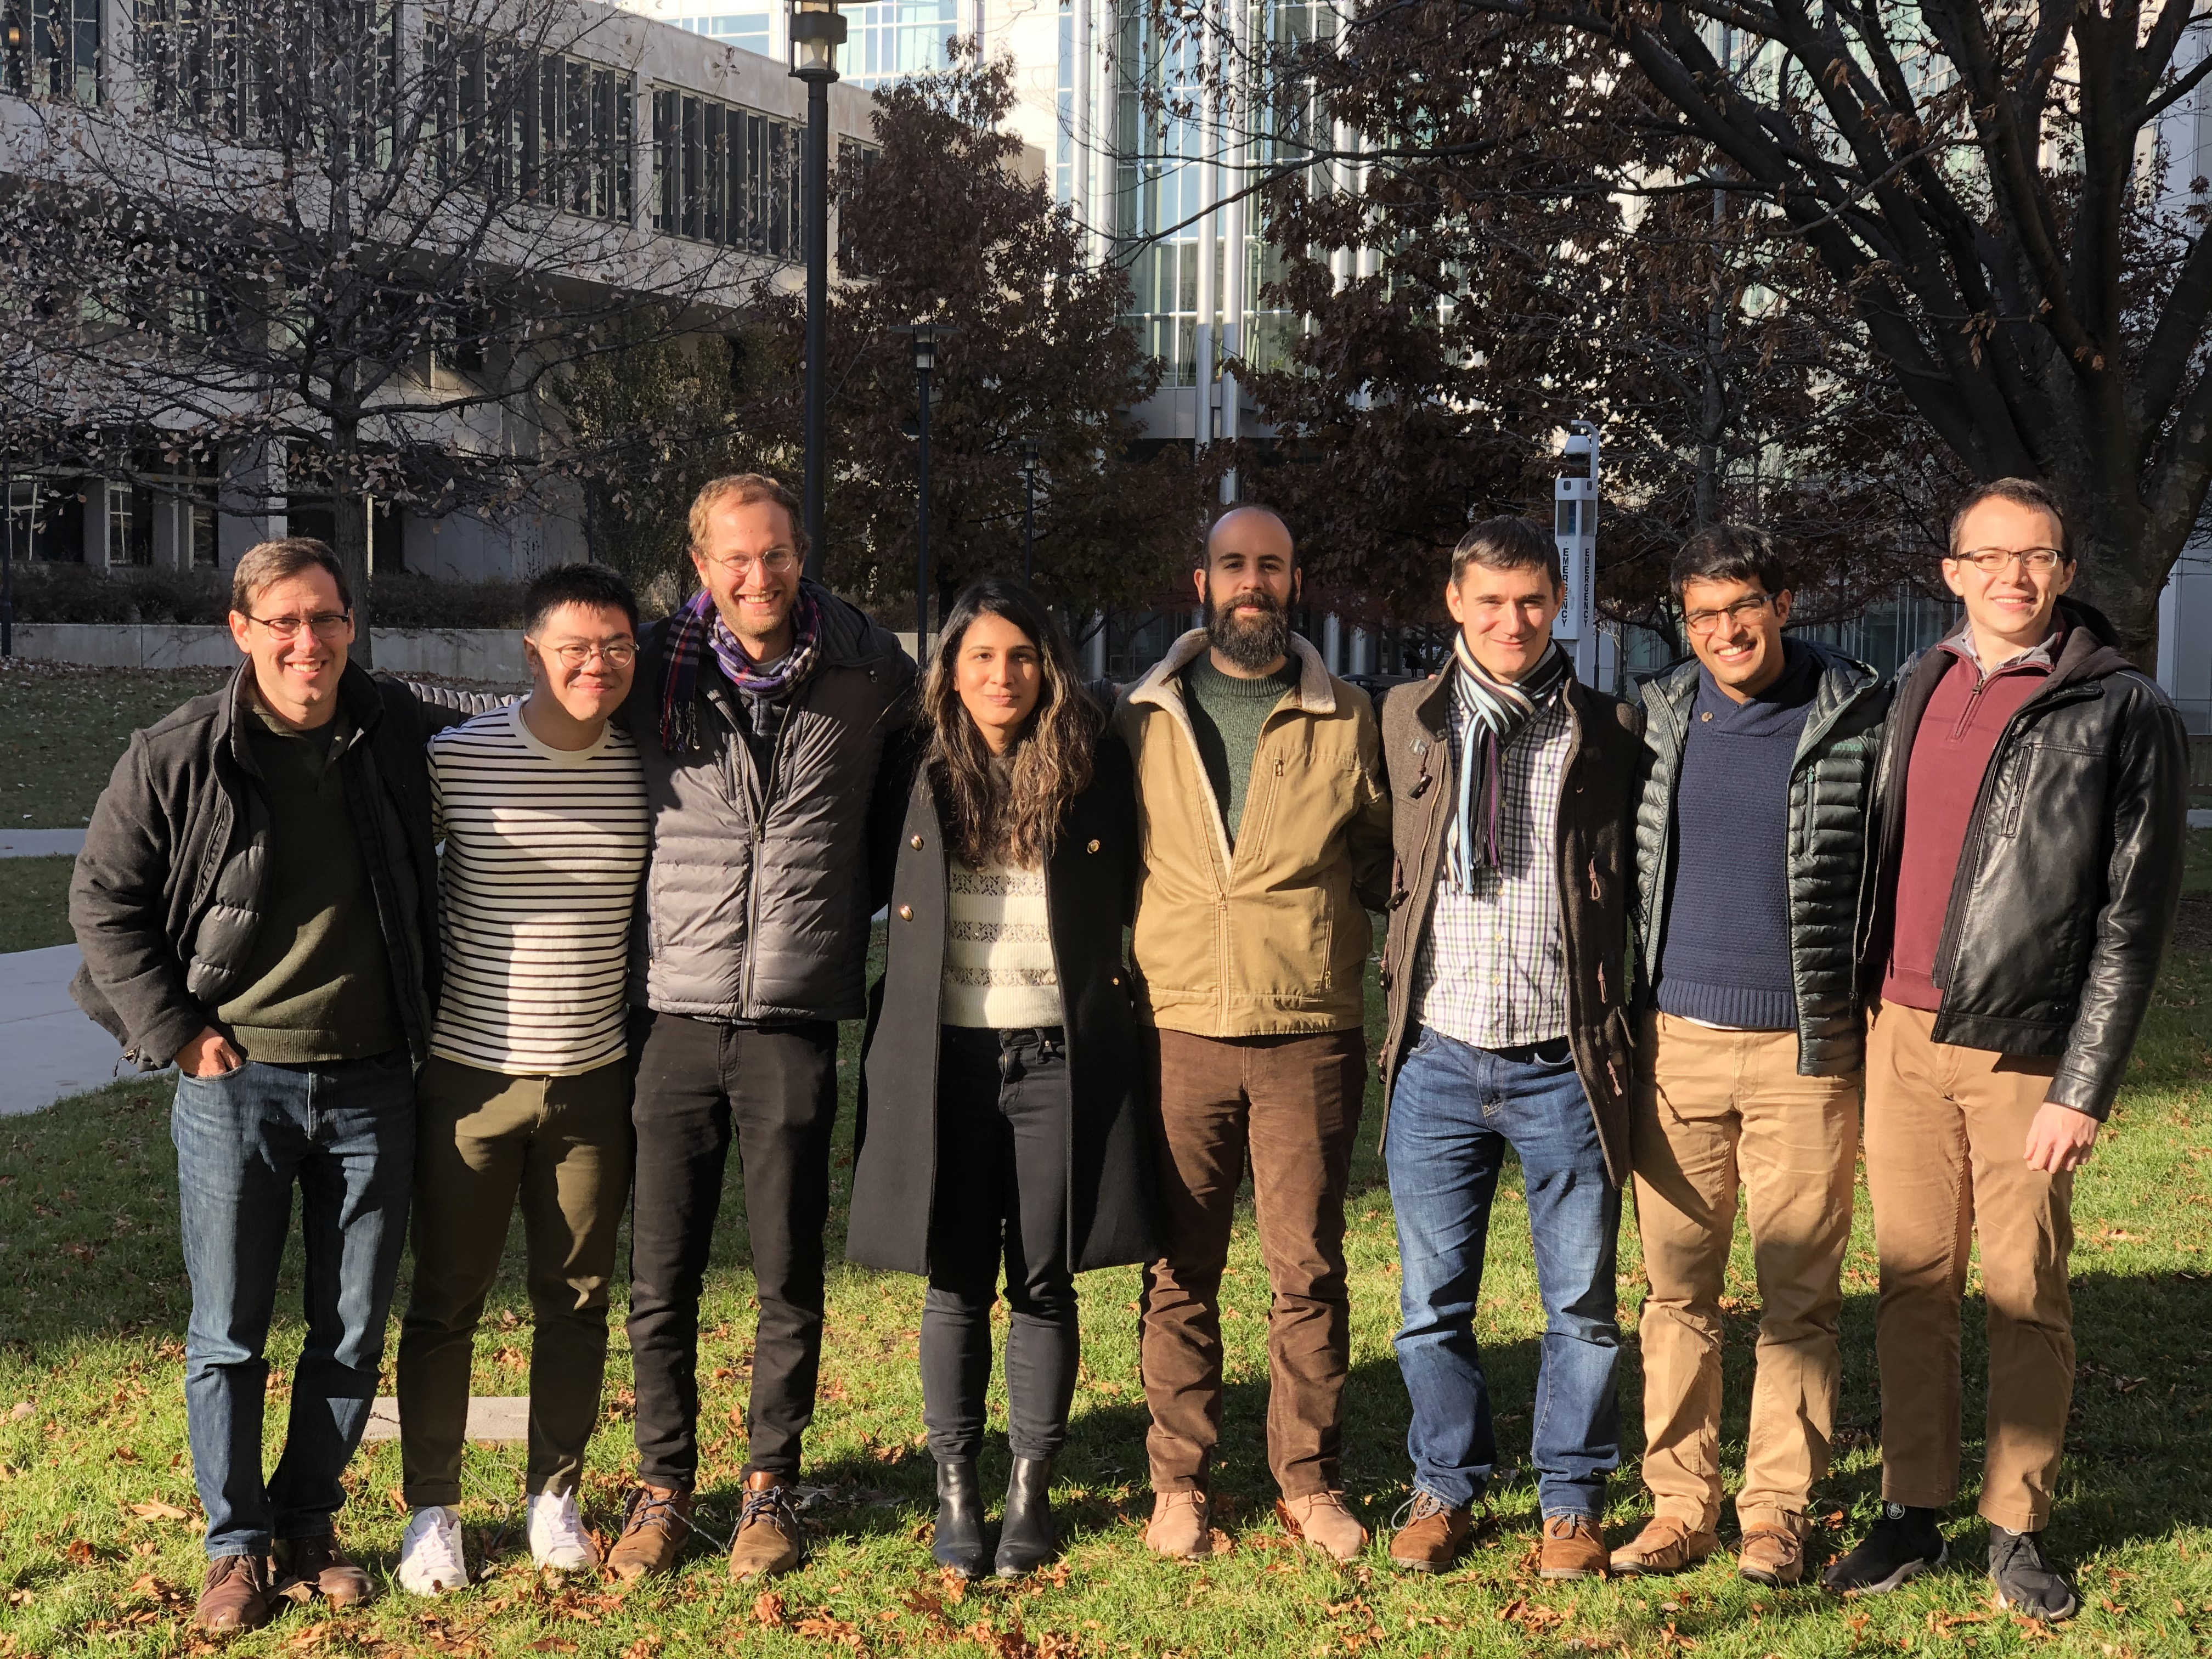
\includegraphics[scale=0.075]{img/IMG_1361.jpg}
    \caption{Novembre lab 2020}
    \label{fig:lab_photo}
\end{figure}


\abstract
% Enter Abstract here
Genome-wide association studies (GWAS) have shown that much of the variation in disease risk is due to rare deleterious alleles. When considering the geographic distribution of a population, studies have shown these alleles are removed by selection before they can spread beyond their original location. However, the geographic distributions of these alleles have not been characterized in detail. This study aims to develop theoretical models to understand how natural selection, geographic structure, and geographic sampling bias interact to determine the inferred local and global genetic architecture of a trait. Our theoretical framework aims to inform the interpretation of GWAS results and quantify the effect of sampling.

\begin{center}
    \textbf{Primary Question:} \\
    How  does geographic sampling bias affect the detection of rare deleterious alleles?
\end{center}


Our primary question can be broken down into the following components:

\begin{enumerate}
    \item Natural selection acts on alleles to determine the traits of a population
    \item Geography influences the distribution of genetic variation 
    \item GWAS identify associated alleles by sampling individuals from particular geographic regions
\end{enumerate}

This dissertation examines these components first from a broad, historical perspective and later through the framework constructed in our theoretical model. The main contribution of this work is an incorporation of geographic sampling process into population genetic models. We relate commonly studied population parameters such as the migration rate $m$ and the selection coefficient $s$ to the observation of rare deleterious alleles from population samples.     

\mainmatter
% Main body of text follows

\chapter{Introduction}
% Introductory stuff
\section{The Foundation of Evolutionary Biology}
Humans have long sought to understand biological variation. To this end, ancient scholars proposed numerous theories of heredity, including that of the \textit{inheritance of acquired characteristics}. It is clear that members of the same family tend to resemble one another. Similarly, members of the same community, or population, tend to share physical characteristics that may be distinct from members of other populations. It is conceivable that children are predetermined to share traits with their parents. Perhaps there exists some quality of living things that allows traits to be recorded throughout one's life and passed down to future generations. Variations in physical characteristics between populations would then be a result of differing records of acquired traits.   

In \textit{On Airs, Waters, and Places}, Hippocrates writes about a community of people known as "Macrocephali" or "Longheads" who would mechanically lengthen the skulls of their children. Hippocrates posits that generations of this practice influenced the natural state of this community such that children were eventually born with long heads without undergoing physical lengthening. 
\begin{quote}
    There is no other race of men which have heads in the least resembling theirs. At first, usage was the principal cause of the length of their head, but now nature cooperates with usage. They think those the most noble who have the longest heads. It is thus with regard to the usage: immediately after the child is born, and while its head is still tender, they fashion it with their hands, and constrain it to assume a lengthened shape by applying bandages and other suitable contrivances whereby the spherical form of the head is destroyed, and it is made to increase in length. Thus, at first, usage operated, so that this constitution was the result of force: but, in the course of time, it was formed naturally; so that usage had nothing to do with it. \cite{hippocrates_airs_waters_places}
\end{quote} 

The inheritance of acquired characteristics remained the predominant explanation of biological variation for more than 2,000 years after Hippocrates. Enlightenment thinkers contributed closely aligned theories with some additional insights, but considerable added terminology. Chief among these are \textit{Lamarckian inheritance} and \textit{Darwinian pangenesis}. Jean-Baptiste Lamarck is famously credited with having developed an evolutionary framework based on the inheritance of acquired characteristics, or "soft inheritance", as he called it.  \cite{lamarck_1914} Lamarck proposed that living things develop in increasing complexity as they adapt to the circumstances of their environment. Novel physical traits arise from their utility to the organism and are subsequently passed on to offspring. Traits that are not of use to the organism are lost. Many young biologists learn of Lamarck's illustration of giraffes stretching and slowly lengthening their necks to reach leaves on trees, leading to subsequent generations with naturally longer necks. This example is often presented as ridiculous when shown in opposition to the \textit{correct} frameworks of Charles Darwin and Alfred Russel Wallace. The theory of evolution by natural selection proposed in \textit{On the Origin of Species by Means of Natural Selection, of the Preservation of Favoured Races in the Struggle for Life} is a fundamental component of modern evolutionary biology. \cite{darwin_1859} Still, Darwin's explanation for heredity was remarkably similar to that of Lamarck and even that of Hippocrates. Darwin's "pangenesis" hypothesis claimed that each part of the body emitted particles of heritable information called "gemmules".\cite{darwin_1868}  If a part of the body was altered in response to one's environment, this part would create altered gemmules. \cite{darwin_pangenesis_1871} These particles were said to aggregate in the gonads to be passed on to offspring.  This hypothesis was invalidated following the rediscovery of Mendelian inheritance in 1900, but the Lamarck-Darwin dichotomy remains a critical teaching construct in biology textbooks. \cite{holterhoff_history_2014} \cite{zirkle_inheritance_1935}


Johann Mendel grew up on a family farm in the village of Hynčice, located in the modern-day Czech Republic. He worked as a gardener during his childhood before obtaining an education in philosophy and physics, but struggled to afford his schooling. Mendel found financial security in joining the Augustinian friars as a monk, adopting the first name "Gregor".  In 1856, Gregor Mendel began studying variation in pea plants after receiving inspiration from his professor Johann Karl Nestler, who studied sheep variation.\cite{henig_2000} He focused on the inheritance of seven discrete characteristics in the common pea plant \textit{Pisum sativum}: seed texture, seed color, pod texture, pod color, flower color, flower position, and plant height. Possible trait variants were indicated by combinations of capital and lower case letters (e.g. \textbf{\textit{Aa}} represented a generation produced by pollination from some round \textbf{\textit{A}} and some wrinkled seeds \textbf{\textit{a}}). The counts of trait appearances across multiple successive generations were recorded, while preventing pollination from foreign plants. Mendel identified several significant principles, coining "recessive" in reference to variants that were observed in preceding and subsequent generations, but masked by other "dominant" variants in some generations. This concept is now referred to as the \textit{Law of Dominance}. Mendel demonstrated that egg and pollen cells carried one of each variant (now called the \textit{Law of Segregation}), and these variants separate independently into egg and pollen cells (\textit{Law of Independent Assortment}). These are all together now known as \textit{Mendel's laws of inheritance}. Mendel's findings were published in the now famous "Experiments on Plant Hybridization" \cite{mendel_1865} in 1866, but were largely ignored until 1900, when his ideas were rediscovered and brought before an incredulous scientific community. The ensuing debate in search of the \textit{correct} mechanisms for biological variation would give rise to modern population genetics. \cite{bowler_2003}

% \subsection{The Mendelian Paradox (possible side discussion)}

%% Maybe include discussion about Mendelian paradox?
%% \cite{fisher_1936}

\newpage
\section{The Modern Synthesis}
The rediscovery of Mendel's work garnered significant attention from early 20th-century biologists. Many scientists saw valuable insight into the mechanisms of heredity by examining Mendel's pea plant experiments. Others argued against the suitability of Mendelian inheritance to explain phenotypic differences on a larger scale. Darwin's work described evolution as a slow process driven by natural selection on small phenotypic differences, while Mendel's showed large, predictable phenotypic differences within a couple generations. Thus began one of the largest controversies in evolutionary biology, the conflict between the "Biometricians" and the "Mendelians." The Mendelians largely supported \textit{saltationism}, or the idea that evolution is driven by large changes between generations. The Biometricians supported \textit{gradualism}, the idea that small and slow changes over time drive evolution. \cire{gilham_2015}


One of the most notable Mendelians was William Bateson, an English scientist largely considered to be one of the founders of genetics. In fact, Bateson is credited with coining the term "genetics" to describe the field. Bateson and British geneticist Edith Saunders published numerous reports analyzing Mendelian inheritance and developed frameworks for understanding evolution based in Mendelian principles. \cite{bateson_1902} The pair even coined the term "allelomorph", or in short "allele" to refer to variants of a gene.  


It was not until Ronald Fisher's 1918 paper "The Correlation between Relatives on the Supposition of Mendelian Inheritance" \cite{fisher_1918} that the Mendelian/Biometrician debate was reconciled. \cite{visscher_r.._2019} Fisher, a brilliant statistician, used mathematics to combine Mendelian inheritance with natural selection and demonstrated how both are compatible with one another. In fact, Fisher claimed that "the sole surviving theory is that of natural selection" on page 20 of his book \textit{The Genetical Theory of Natural Selection}.  \cite{fisher_1930} Fisher's contributions formed the basis of the "Modern Synthesis" of evolutionary biology. The restructuring of theoretical frameworks toward a unified theory of evolution. The term was coined by evolutionary biologist and outspoken eugenicist Julian Huxley in his 1942 book, \textit{Evolution: The Modern Synthesis} \cite{huxley_1942}. Like Huxley, Fisher often argued on behalf of eugenics. The final chapter of Fisher's \textit{The Genetical Theory of Natural Selection} describes his concern with allowing members of human civilization with less than desirable traits to pass on those traits to future generations. Nevertheless, Fisher's work marked a turning point in our collective understanding of biological variation. His insights remain a driving force for new discoveries.


Fisher, J.B.S. Haldane, and \textcolor{maroon}{University of Chicago} geneticist Sewall Wright are considered to be the founders of the field of population genetics. Population geneticists study genetic differences in and between populations with an often "first principles" approach. The contributions of population genetics tend to be theoretical and mathematical in nature, coercing complex systems like the dynamics of molecular evolution or the identification of multiple coalescent events into models and equations \cite{rice_2016} \cite{rice_2018}. Population genetics is a highly interdisciplinary field, connecting across biology into math, statistics, physics, computer science, and others to understand the forces of nature that shape populations. Truly a rich and exciting field. \cite{gillespie}

\section{Genes and Geography}
While much of evolutionary theory deals with change over time, populations interact 

Isolation by distance

Novembre et. al.2008


Novembre and Stephens 2008 human genetic data shows continuous spatial structure 


A note on
: Allison Etheridge on Spatial modeling in popgen 

\section{GWAS and Sampling Processes}
The genomics revolution & GWAS


Bias in genomic data collection


The Site Frequency Spectrum as a quantitative summary of segregating sites 


Sampling process distorts important quantities in popgen analyses --- SFS

McVean 2009, Battey 2019 

\newpage
\section{Project Rationale and Significance}
%% Need to reformat citations!
Quantitative and population geneticists are interested in finding statistical associations between genetic variants and particular traits. Genome-wide association studies (GWAS) are one common method for detecting associations and are especially useful when attempting to predict an individual’s risk for disease. Disease GWAS function by comparing a large set of genotypes to the known disease phenotypes of members in the group. If members with a particular allele, or variant of a gene, are shown to have a significantly higher probability of also being in the group with the disease, then the GWAS supports the hypothesis that the allele increases one’s risk of developing the disease. GWAS typically estimate the genetic effects on a phenotype by conducting a linear regression as follows:\cite{dudbridge_2013} \cite{xie_xu_1998}

\begin{equation}
    \hat{\bf{Y}} = \boldsymbol{\hat{\beta}} \bf{G} + \boldsymbol{\epsilon} = \sum_{i=1}^{n} (\hat{\beta_i} G_i + \epsilon_i) 
\end{equation}

Where $\hat{\bf{Y}}$ represents the phenotype expressed as a linear combination of $n$ genetic loci in matrix $\bf{G}$ scaled by their effect sizes $\hat{\beta}$. Error terms are accounted for in $\boldsymbol{\epsilon}$ and are independent from $\bf{G}$. It is important to note that $\hat{\beta}$ is an estimated quantity. Researchers have proposed a number of statistical methods for estimating effect sizes. \cite{meuwissen_etal._2001} \cite{park_etal._2011}



Conducting a GWAS requires a large set of genomic data which is gathered by a sampling process. As a result, association studies feature significant geographic sampling bias. For example, the UK BioBank contains samples of people who have migrated to the United Kingdom from around the world, but still represents a small fraction of global diversity [?]. Therefore, it is important to assess if GWAS results from geographically localized studies, such as those from the UK BioBank, can predict disease risk in other geographic regions. This project adds to the existing literature of theoretical models for studying deleterious alleles [8][9][10], but is one of the first to consider the influence of spatial sampling bias. Then, the goal of this project is to create a framework for evaluating how geographic sampling bias may affect the detection of rare deleterious alleles. Towards these ends, we note the following aims:	

\begin{enumerate}
    \item Develop theoretical models to derive the distribution of allele frequencies as a function of the spatial sampling scheme.
    \item Determine the effect of sampling schemes on allele detection probability.
\end{enumerate}


Preliminary studies have shown that deleterious, disease-causing alleles or those with large effects are often rare \cite{marouli_rare_2017} \cite{slatkin_estimating_2000}, and rare alleles are often geographically localized \cite{visscher_r.._2019}\cite{slatkin_spatial_1978}. Through an evolutionary biology lens, we expect deleterious alleles to be removed from a population by natural selection before they can spread far from their location of origin. The rate at which these alleles are removed depends on how deleterious the allele is. Alleles with large deleterious effects are hypothesized to be removed much faster by selection, and therefore be kept rare in a population. As a result, we expect this allele to exist in a relatively small geographic region. Whereas alleles with small effect sizes are expected to span wider regions and exist at higher frequencies. 

\begin{figure}[h]
    \centering
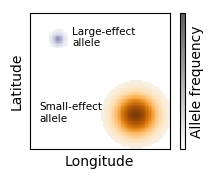
\includegraphics[scale=1.5]{img/spatial_distributions.png}
    \caption{This schematic illustrates the geographic distribution of alleles with varying effect sizes. Large effect, or strongly deleterious alleles are kept at low frequencies and are more geographically isolated due to natural selection. Small effect alleles are found in wider regions and at higher frequencies.}
    \label{fig:spatial_schematic}
\end{figure}


As mentioned previously, GWAS cohorts tend to be geographically localized. This is attributed mostly to convenience and limitations in resources. Researchers do not \textit{yet} have the capacity to sequence all members of a population in all locations, and pooling genomic data from multiple studies may create biased results subject to batch effects. \cite{woolston_2015}\cite{gilad_2015} Therefore, the detection of rare deleterious alleles is especially challenging for GWAS. The ability to detect large-effect alleles is dependent upon process by which researchers sample individuals to sequence. Not only is there a lower probability of sampling individuals with the allele of interest, but small-effect alleles can mask the detection of large-effect alleles. Even if some individuals with the allele of interest are sampled, smaller-effect alleles can comprise a larger proportion of the sample, making large-effect allele detection difficult. There exists a trade-off between sampling individuals in a narrow geographic region, and sampling the same number of people from a broader region. For the former, such a GWAS is more likely to find no associations (landing exclusively in the white space of Figure \ref{fig:spatial_schematic}. While for the latter, such a GWAS may find some of the large-effect allele of interest, but is more likely to not have enough representation in the sample to detect the rare allele. 


A theoretical framework describing the geographic distribution of rare deleterious alleles could help optimize sampling strategies for GWAS cohorts. However, there does not yet exist a framework that considers the interactions between the evolutionary forces acting upon an allele and the sampling process that influences which alleles are detectable. This project aims to construct such a framework. We will utilize population genetic theory and simulations to examine the geographic distribution of rare deleterious alleles. 


This work is ultimately interested in understanding how the process of sampling may affect the power of a GWAS to detect deleterious alleles, as this interaction has not been previously studied. This theoretical framework aims to inform the interpretation of GWAS results and quantify the effect of sampling. The project aims to relate the power to detect disease-causing alleles to the evolutionary forces acting upon them and the constructed sampling scheme. It is predicted that certain sampling schemes may increase the power of a GWAS for certain alleles. The model proposed allows one to quantitatively determine the optimal sampling strategies for given deleterious alleles of varying rarity. This model can ultimately be used to inform future GWAS study design by accounting for sampling effects in data collection, possibly increasing the power of a GWAS to detect rare alleles. This could likely improve GWAS predictions of individual disease risk.


\begin{center}
    \textbf{Primary Question:} \\
    How  does geographic sampling bias affect the detection of rare deleterious alleles?
\end{center}

\chapter{Methods}

\section{Theoretical Models}

Our model is based on the classic Wright-Fisher [3][4] and Stepping Stone [5] population genetic models which describe evolution and migration, respectively. In this section, we present the logic of these models using the parameterization best suited for our purposes. Namely, we consider a \textit{haploid} population of size $N$ as opposed to a \textit{diploid} population. However, much of the following derivations are applicable to diploid models. The modified derivations largely follow the logic of the original Wright [3] and Kimura [5] papers, with some more modern insights.\cite{Rackauckas2014AnII}\cite{tran_2012} \cite{durret_2008}


\subsection{The neutral Wright-Fisher model} \label{section:neutral_wf}

The neutral Wright-Fisher model [3][4], named after population geneticists Sewall Wright and Ronald Fisher, considers an idealized population with random mating, non-overlapping generation times; and without mutation, migration or natural selection. Despite these assumptions, the model serves as a useful tool for studying evolutionary forces acting upon a population, particularly genetic drift. More complex evolutionary forces can be incorporated seamlessly, as our work will show. 


We start by considering a \textit{haploid} population of finite size $N$ and a single genetic locus with two alleles, $A$ and $a$. The total population size remains constant. Let $X_t$ be the number of $A$ alleles at generation $t$.Therefore, the frequency of $A$, $f_t$, is simply:

\begin{equation}
    f_t = \frac{X_t}{N}
\end{equation}

This implies that the frequency of $a$ is simply $1-f_t$. So we only need to keep track of changes to $f_t$. We call $A$ the "focal allele". Alleles are passed on to the next generation $t+1$ independently of one another, via sampling with replacement. We want to know the probability of having $k$ copies of allele $A$ in the next generation, where $k \in \{0,1,...,N\}$. To learn this, we need to know how $X_{t+1}$ is distributed. Because the choice between the two alleles is independent of one another, and because we are sampling with replacement:

\begin{equation}
    X_{t+1} \sim Binomial(N,f_t)
\end{equation}

 The probability mass function of the binomial distribution gives the following result:

\begin{equation}
    P(X_{t+1} = k) = {N \choose k}(f_t)^k (1-f_t)^{N-k}
\end{equation}

This describes the probability of transitioning from $X_t$ number of alleles to $X_{t+1} = k$ number of alleles in one generation, or from $f_t$ to $f_{t+1}$. This \textit{Markov} process begins with a given initial frequency $f_0$ and repeats for each generation. 


We will continue by describing some properties of this model. The expected value of $E[X_{t+1}]$ is shown using the Law of Total Expectation.

\begin{equation} \label{eq:ex_drift}
    \begin{split}
            E[X_{t+1}] &= E[E[X_{t+1}|X_{t}]] = E[N f_t] = E[X_t] \\
    \implies E[f_{t+1}] &= E[f_t] = f_0
    \end{split}
\end{equation}


The average allele frequency is determined by the set initial allele frequency. We can think of this process as a random walk starting at $f_0$ with equal probability of stepping towards 1 or 0 with an overall average of $f_0$. What is the variance of this random walk? Because the expected value of $f$ at the next generation is equal to the value at the current generation, $f$ is known as a \textit{martingale} by definition. The variance of a martingale is thus:
 
\begin{equation}
    \begin{split}
            Var[X_{t+1}] &= N f_t(1-f_t) \\
            \implies Var[f_{t+1}] &= Var[\frac{X_{t+1}}{N}] =  \frac{1}{N^2} N f_t(1-f_t) = \frac{f_t (1-f_t)}{N} 
    \end{split}
\end{equation}

We also get this definition from the variance of a binomial random variable. 


Notice that the variance in the focal allele frequency between generations is dependent on the population size. This reflects an empirically observed property of genetic drift. Small populations experience larger variation in allele frequencies per generation than large populations. The following holds:

\begin{equation}\label{eq:var_lim_drift}
    \lim_{N \to \infty} Var[f_{t+1}] = 0
\end{equation}

We want to capture these dynamics in a single equation. One reason for this is that single equations are simpler to write and thus are simpler to simulate and analyze. However, the inclusion of randomness in our model prohibits the use of ordinary differential equations (ODEs) like those commonly written to describe change in more deterministic systems in biology. We will use stochastic calculus to arrive at such an equation.


If we assume $N$ to be large, we can consider changes in allele frequencies due to genetic drift to be almost continuous and differentiable. Therefore, we can write an equation of the form: 

\begin{equation}
    df_t = \mu_t \, \,dt + \sigma_t \, \,dB_t
\end{equation}


This equation is a \textit{stochastic differential equation} (SDE) that represents the change in allele frequencies over time. We see a term $\mu_t \, \, dt$ that resembles the form of an ODE, but unlike an ODE we have an added $dB_t$ term scaled by $\sigma_t$. SDEs generalize ordinary differential equations by adding a random Brownian noise term $dB_{t}$. In an infinitesimal time interval $dt$, the noise has mean $0$ and variance $dt$. Solutions to SDEs are probability densities rather than functions of time or space, as with an ODE. There exists a well-developed body of theory for solving SDEs in stochastic calculus. One of the theoretical contributions most relevant to this project is \textit{It\^{o}'s lemma}, named after Japanese Mathematician Kiyosi It\^{o}. \cite{ito_1944} We will use the lemma to demonstrate exactly what $\mu_t$ and $\sigma_t$ represent. Then we will find the correct $\mu_t$ and $\sigma_t$ for the Wright-Fisher model. 


For some function $g(f_t)$ It\^{o}'s lemma gives:

\begin{equation}
    \begin{split}
        dg(f_t) 
                &= \frac{dg}{df_t}df_t + \frac{1}{2} \frac{d^2g}{df_t^2}(df_t)^2 + ... \\
                &= (\frac{\partial g}{\partial t} + \mu_t \frac{\partial g}{\partial f_t} + \frac{\sigma_t^2}{2} \frac{\partial^2 g}{\partial f_t^2})dt + \sigma_t \frac{\partial g}{\partial f_t}dB_t \\
                &= (\mu_t \frac{\partial g}{\partial f_t} + \frac{\sigma_t^2}{2} \frac{\partial^2 g}{\partial f_t^2})dt + \sigma_t \frac{\partial g}{\partial f_t}dB_t \\
    \end{split}
\end{equation}


This is essentially an extension of the chain rule for SDEs. The $\frac{\partial g}{\partial t} \to 0$ as $g$ is not a function of $t$. This formulation allows us to examine the expected values $E[g(f_t)]$ for given functions $g$. Note the following and recall that $E[dB_t] = 0$:

\begin{equation}
    E[dg(f_t)] = (\mu_t \frac{\partial g}{\partial f_t} + \frac{\sigma_t^2}{2} \frac{\partial^2 g}{\partial f_t^2})dt
\end{equation}


Let $g(f_t) = f_t$. This implies $\frac{\partial g}{\partial f} = 1$ and $\frac{\partial^2 g}{\partial f^2} = 0$.


\begin{equation}
    \begin{split}
         E[dg(f_t)] &= E[df_t] = (\mu_t \times 1 + \frac{\sigma_t^2}{2} \times 0)dt \\
         & \therefore \mu_t = \frac{E[df_t]}{dt} = \frac{d}{dt}E[f_t]
    \end{split}
\end{equation}


Leibniz's rule allows us to pull the $\frac{d}{dt}$ out of the expectation. 


We now have our $\mu_t$ for the model. $\mu_t$ is defined as the \textit{infinitesimal mean}, or how much the average allele frequency changes at each instant. Recall that we set a constant initial frequency value $f_0$. For the Wright-Fisher model, we have $E[f_t] = f_0$. This implies that $\mu_t = \frac{d}{dt} (f_0) = 0$. Let us now solve for $\sigma_t$.


Similarly, we define $g(f_t) = (f_t - f_0)^2$. This implies that $\frac {\partial g}{\partial f} = 2(f_t - f_0)$ and $\frac{\partial^2 g}{\partial f^2} = 2$.


\begin{equation}
    \begin{split}
         E[dg(f_t)] &= E[d(f_t-f_0)^2] = (\mu_t \times 2(f_t - f_0) + \frac{\sigma_t^2}{2} \times 2)dt \\
         \implies \sigma_t &= \sqrt{\frac{E[d(f_t-f_0)^2]}{dt}} = \sqrt{\frac{d}{dt}E[(f_t-f_0)^2]} \\
         &= \sqrt{\frac{d}{dt}E[(f_t-E[f_t])^2]} = \sqrt{\frac{d}{dt}Var(f_t)}
    \end{split}
\end{equation}


We see that $\sigma_t$ is the \textit{infinitesimal standard deviation}, or the square root of the infinitesimal variance. This represents how far we expect the allele frequency to deviate from the mean at each instant. The SDE is a continuous-time approximation of the discrete-time Markov process we wrote initially. Therefore, we take the limit as $\Delta t \to 0$. The recursive solution of $Var[f_t]$ previously shown becomes:

%% skip Kolmogorov Forward equation

\begin{equation}
    \begin{split}
         Var[f_t] &= \frac{f_{t-1}(1-f_{t-1})}{N} \\
         \implies \frac{d}{dt} Var[f_t] &= \frac{f_t(1-f_t)}{N} \\
         \therefore \sigma_t &= \sqrt{\frac{f_t(1-f_t)}{N}}
    \end{split}
\end{equation}

Finally, we arrive at an SDE for the neutral Wright-Fisher model. This SDE has mean and standard deviation equal to the solved $\mu_t$ and $\sigma_t$. We drop the subscript $t$ for clarity, noting that this SDE describes continuous change over time. 

\begin{equation}
    df = \sqrt{\frac{f(1-f)}{N}} dB_t
\end{equation}


We can incorporate additional evolutionary forces simply by adding terms to the Wright-Fisher SDE above as one would for an ODE. Section \ref{"section:our_model"} shows the expanded Wright-Fisher SDE that we use to simulate more complex evolution. 


\subsection{The Stepping Stone model}

A population spread over a large area will experience often noticeable differences between members of different local territories. Species tend to form clusters, and different clusters tend to have unique differences. We expect these clusters, or demes (sub-populations), to be more different from one another the farther apart they are along the total range of the population. Migration occurs more easily between nearby demes, allowing for interbreeding and more similar genetic  backgrounds. A number of theoretical models have been proposed to capture this process.\cite{wright_1943} \cite{malecot_1959} This section will examine the classic Stepping Stone model. 

The Stepping Stone model was first presented by Japanese population geneticist Motoo Kimura in 1953. \cite{kimura_1953} In fact, this paper was Kimura's first population genetics publication. \cite{crow_1994} The model considers the distribution of allele frequencies over an array of demes connected by migration. We consider one spatial dimension. 

\begin{figure}[h]
    \centering
    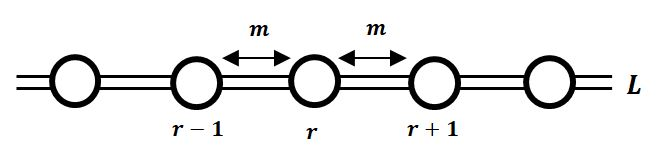
\includegraphics[scale=0.8]{img/model_schematic.JPG}
    \caption{This schematic represents the geographic structure for the model in one dimension. Circles represent demes which are indexed by integer $r$. There are $L$ many demes connected to nearest neighbors via a migration rate $m$. The boundaries are connected to one another, effectively creating a \textit{ring} of demes.}
    \label{fig:schematic}
\end{figure}


Allele frequencies change in each deme over time. We assume that change occurs in discrete generation time. For a single locus with two alleles $a$ and $A$, let $f_r$ be the current allele frequency of $A$ at deme $r$. The allele frequency in this deme at the next generation $f_r'$ is the following:

\begin{equation}
    f_r' = (1-2m-m_\infty)f_r + m(f_{r-1} + f_{r+1}) + m_\infty \bar{f} + \xi_r
\end{equation}


Where $m$ is the symmetric migration rate connecting neighboring demes. $2m$ represents the rate at which individuals in deme $r$ move to the two neighboring demes. $m_\infty$ represents "long range dispersal". Kimura and Weiss (1964) \cite{kimura_1964} describes this as the rate by which individuals enter new demes as a random sample of the entire population where the probability of sampling $A$ is $\bar{f}$, the frequency of $A$ averaged over each deme. $m_\infty$ is mathematically equivalent to mutation. $\xi_r$ describes random changes in frequency due to genetic drift. As seen in the Wright-Fisher model, $\xi_r$ is a binomial random variable with mean $E[\xi_r]=0$ and $Var[\xi_r] = \frac{f_r(1-f_r)}{N}$ (or $2N$ for a diploid population).


For now, we focus only on migration between nearest neighbors so we ignore $m_\infty$. We also assume $N$ is large in each deme, so that $\xi_r \to 0$. Therefore, we can rearrange terms to arrive at the linear difference equation:

\begin{equation}
    \begin{split}
        f_r' &= (1-2m)f_r + m(f_{r-1} + f_{r+1}) \\ 
        f_r' &= f_r -2mf_r + m(f_{r-1} + f_{r+1}) \\
        f_r' - f_r &= m(f_{r-1} + f_{r+1} - 2f_r)
    \end{split}
\end{equation}


This equation demonstrates the difference in per-generation allele frequency in each deme. As $\Delta t \to 0$, we can show the continuous form:

\begin{equation}
    \frac{df_r}{dt} = m(f_{r-1} + f_{r+1} -2f_r)
\end{equation}

which describes the continuous change over time due to migration. 


Note the expected value $E_t[E_r[df_r]]$ averaged over position $r$:

\begin{equation}
    \begin{split}
        E_r[df_r] &= m(E_r[f_{r-1}] + E_r[f_{r+1}] -2E[f_r])dt \\
        &= m(f+f-2f) = 0 \\
        \implies E_t[E_r[df_r]] &= 0 
    \end{split}
\end{equation}


On average, migration does not influence the changes in allele frequency. 


We can expand the model to two spatial dimensions. This gives an interconnected lattice of demes. Let us only allow for nearest-neighbor migration along cardinal directions, i.e. we allow for individuals in each deme to move along two axes $r$ and $s$:

\begin{figure}[h]
    \centering
    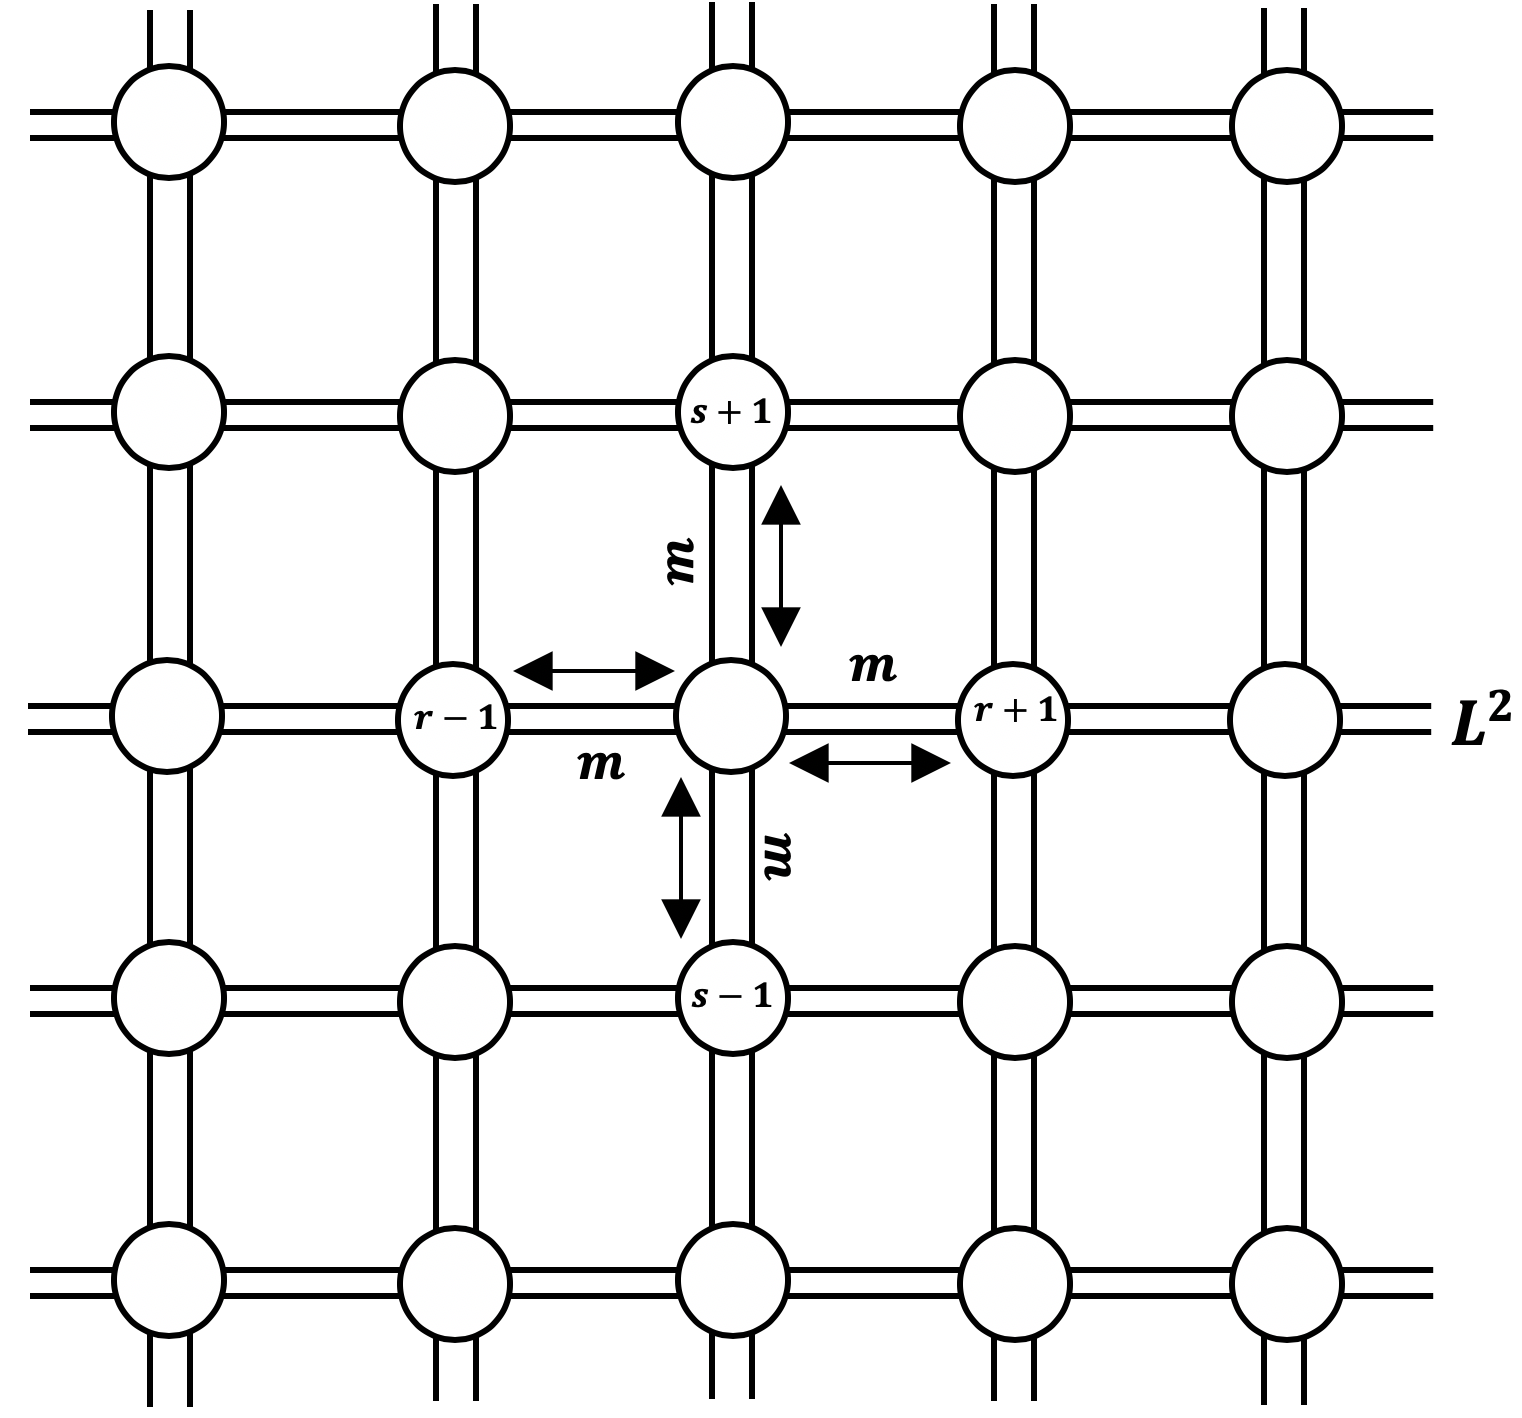
\includegraphics[scale = 0.3]{img/2d_ss.png}
    \caption{The two-dimensional Stepping Stone model with $L^2$ demes. We allow for symmetric migration at rate $m$ between nearest neighbors. Positions on the grid are shown by $r$ along the horizontal axis and $s$ along the vertical axis.}
    \label{fig:2d_ss}
\end{figure}


We can write $df_{r,s}$ for the two-dimensional model by simply expanding the form of $df_r$ as shown:


\begin{equation} \label{eq:stepstone}
    df_{r,s} = m(f_{r-1,s} + f_{r+1,s} + f_{r,s+1} + f_{r,s-1} - 4f_{r,s})dt
\end{equation}


Note that $E[df] = 0$ in two dimensions as well. The Stepping Stone model provides a useful framework for understanding the influence of migration on evolution. In the next section, we expand upon this framework to incorporate more complex evolutionary forces acting on alleles distributed over the geographic lattice.  


\subsection{Our model} \label{"section:our_model"}

As mentioned previously, our model combines the classic Wright-Fisher and Stepping Stone models. We describe the allele frequency in a finite population of $N$ individuals grouped into discrete \textit{demes} connected by migration (Figure \ref{fig:schematic}). Each deme is occupied by a fixed, constant population size, which regulates the local population density \cite{felsenstein_1975}. We consider a single genetic locus with two alleles. The focal allele frequency in each deme is $f_r$ with $r$ indexing deme location. Allele frequencies change according to four evolutionary forces:


\begin{enumerate}
    \item \textbf{Mutation} changes one allele to another at rate $\mu$
    \item \textbf{Natural selection} reduces the frequency of the deleterious allele at rate $s$
    \item \textbf{Migration} reduces the allele frequency differences between nearby demes at rate $m$
    \item \textbf{Genetic drift} introduces random noise in a finite population at rate $\frac{1}{N}$, \\ where $N$ is the population size
\end{enumerate}


The change in allele frequency in each deme $df_r$ is described by the following stochastic differential equation:

\begin{equation}
    \label{eq:model}
    df_r=[\mu(1-2f_r)-sf_r (1-f_r ) + m (f_{r-1}+f_{r+1}-2f_r)]dt+\sqrt{\frac{f_r (1-f_r )}{N}} dB_{t,r}
\end{equation}


Note that we consider a symmetric migration rate. The rate at which individuals leave their current deme is the same as the rate at which individuals enter that deme. We also consider a symmetric mutation rate. The rate at which allele $a$ changes into $A$ is the same as the reverse mutation. Loci are modeled as independent replicates.

While these models have been studied extensively [14][15][16], most work has been focused on neutral evolution. A caveat to this is the study of "clines", or measurable gradients of biological characteristics across geographic ranges. Some population geneticists and evolutionary biologists have studied changes in clines in situations of non-neutral evolution. \cite{baines_2004} Still, many of these studies still focus on examining the influence of genetic drift on cline patterns. \cite{polechova_barton_2011} The main difference between the theory of clines and the non-neutral evolutionary theory we propose, is that cline theory is concerned with the \textit{mean} allele frequency, while we are concerned with the \textit{distribution} of allele frequencies.\cite{vasemagi_2006} This distribution is more relevant for rare alleles and large samples. 


Expanding the Wright-Fisher model allows us to examine allele frequencies acted upon by each of the four evolutionary forces. We simulate the evolution of rare deleterious alleles over many generations and over large geographic environments. Using this equation, important information about the evolution of rare deleterious alleles can be discovered. In the next chapter, we will derive important quantities that describe the average number of rare allele copies as a function of the evolutionary parameters along with the quantity describing the average geographic range of an allele. We will also describe the expected distribution of allele frequencies across demes, known as the \textit{Site Frequency Spectrum}.


Our approach involves first simulating the underlying distribution of allele frequencies, and second, sampling from this distribution using a variety of sampling scheme. Our subsequent analysis examines the information loss as a function of sampling. We are interested in the interaction between the process of sampling and the "unobserved" underlying frequency distribution. 

\begin{figure}[h]
    \centering
    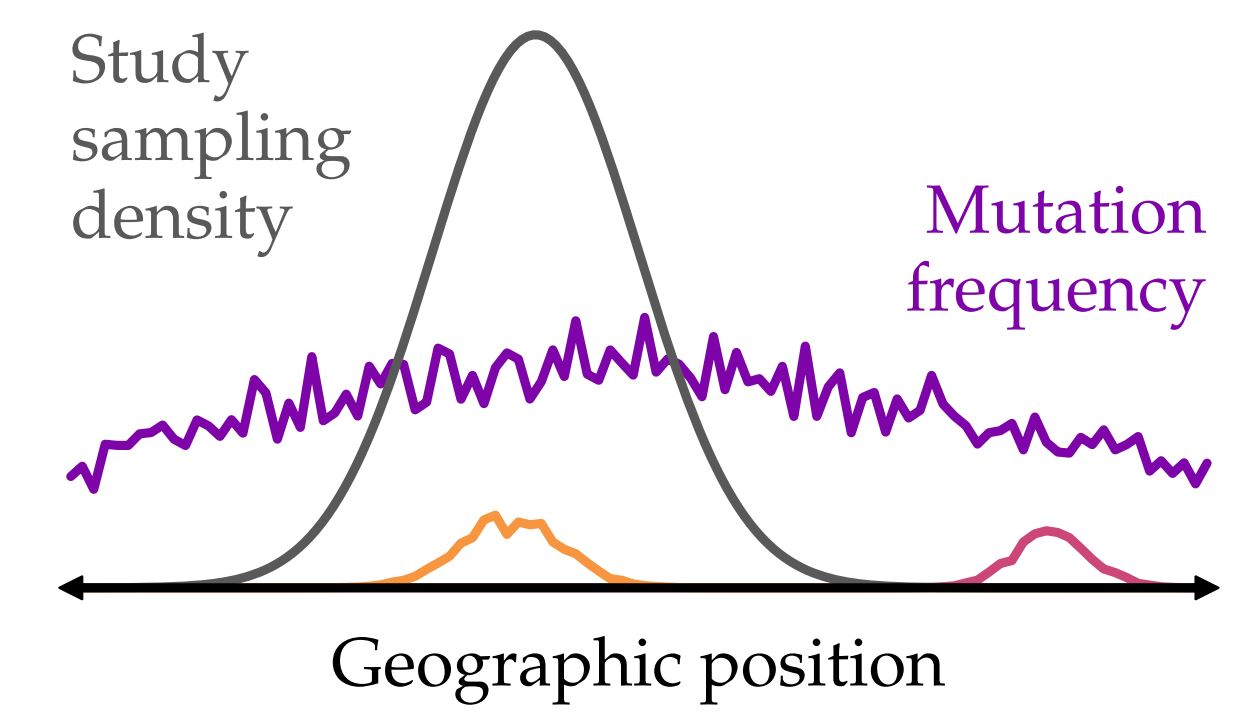
\includegraphics[scale=0.4]{img/smapling_schematic.JPG}
    \caption{This schematic illustrates the interaction between the underlying allele frequency distribution and the sampling scheme imposed by an association study. We see that alleles are typically confined to a range of geographic positions, with rare alleles having a smaller range. We expect the distribution of alleles observed in a GWAS to depend on the location of the sampling distribution relative to the allele frequency distribution.}
    \label{fig:sampling_schematic}
\end{figure}

\newpage
\section{Simulations}

This section describes the various tools used to simulate our model. In theory-based research, simulations are important for several reasons. First, they allow us to observe a system that is typically too complex to study empirically. The evolutionary history of life spans billions of years. Simulations allow us to study evolution over thousands of generations in a matter of seconds. Second, simulations allow us to validate theoretical predictions made by our model. We can derive properties of our system analytically, and show that these properties hold computationally. Much of our project results come from first making predictions based on our model, and then confirming these predictions with simulations. Hundreds of simulations have been run throughout the course of this project, producing hundreds of gigabytes of data. The University of Chicago Research Computing Cluster has made this process possible. All code presented in this section is available by request at github.com/dp-rice/spatial-simulations. 


Our simulations were designed using two distinct frameworks: 

\begin{enumerate}
    \item \code{SLiM} ("\textbf{S}election on \textbf{Li}nked \textbf{M}utations")
    \item \code{NumPy} arrays and custom-written functions in \code{Python}
\end{enumerate}

\code{SLiM} is a simulation package for population genetics designed by Phillip Messer and Benjamin Haller at Cornell University in 2013.\cite{slim} The package contains a broad range of functionality for simulating the evolution of complex systems. Researchers have used \code{SLiM} to investigate the dynamics of population bottlenecks \cite{pederson_2017}, ancient human migration \cite{sikora_2017}, regional heritability mapping \cite{caballero_2015}, and much more. The versatility of \code{SLiM} allows for whole-genome simulations, continuous spatial models, age structure. For our purposes, this added functionality proved unnecessary and we chose to write our own simulation programs in \code{Python}.  

\code{NumPy} ("\textbf{Num}erical \textbf{Py}thon extensions") is the staple \code{Python} package for working with large sets of numerical data. The package demonstrates superior computational efficiency, both in terms of processing speed and memory usage. \code{NumPy} is at the core of much scientific computing.\cite{numpy} We use the package to efficiently create, manipulate, and store arrays of simulation data. The following sections demonstrate our process. 


\subsection{Evolution in discrete space}

Recall that our SDE model describes the change in allele frequencies over time in discrete demes connected by migration:

\begin{equation}
    \tag{\ref{eq:model} revisited}
    df_r=[\mu(1-2f_r)-sf_r (1-f_r ) + m (f_{r-1}+f_{r+1}-2f_r)]dt+\sqrt{\frac{f_r (1-f_r )}{N}} dB_{t,r}
\end{equation}

Our simulations use this equation to generate changes in allele frequencies over time, given an initial allele frequency $f_0 = \frac{1}{N}$ and a set of population parameters. We begin with a one deme population ($L = 1$) and the following parameters:

\lstinputlisting[language=iPython, caption = Population parameters, label = code:params]{src/param_list.py} 

Our simulation output contains a vector of allele frequency values for every generation. We perform many independent replicates of each trajectory to represent multiple loci and compute statistics from our data. The figure below shows an example stochastic trajectory of allele frequencies over time. With purifying natural selection (large $s$), the allele remains rare as $s$ determines the rate at which the allele is removed from the population. We observe this to be the case in the example shown.


\begin{figure}[h]
    \centering
    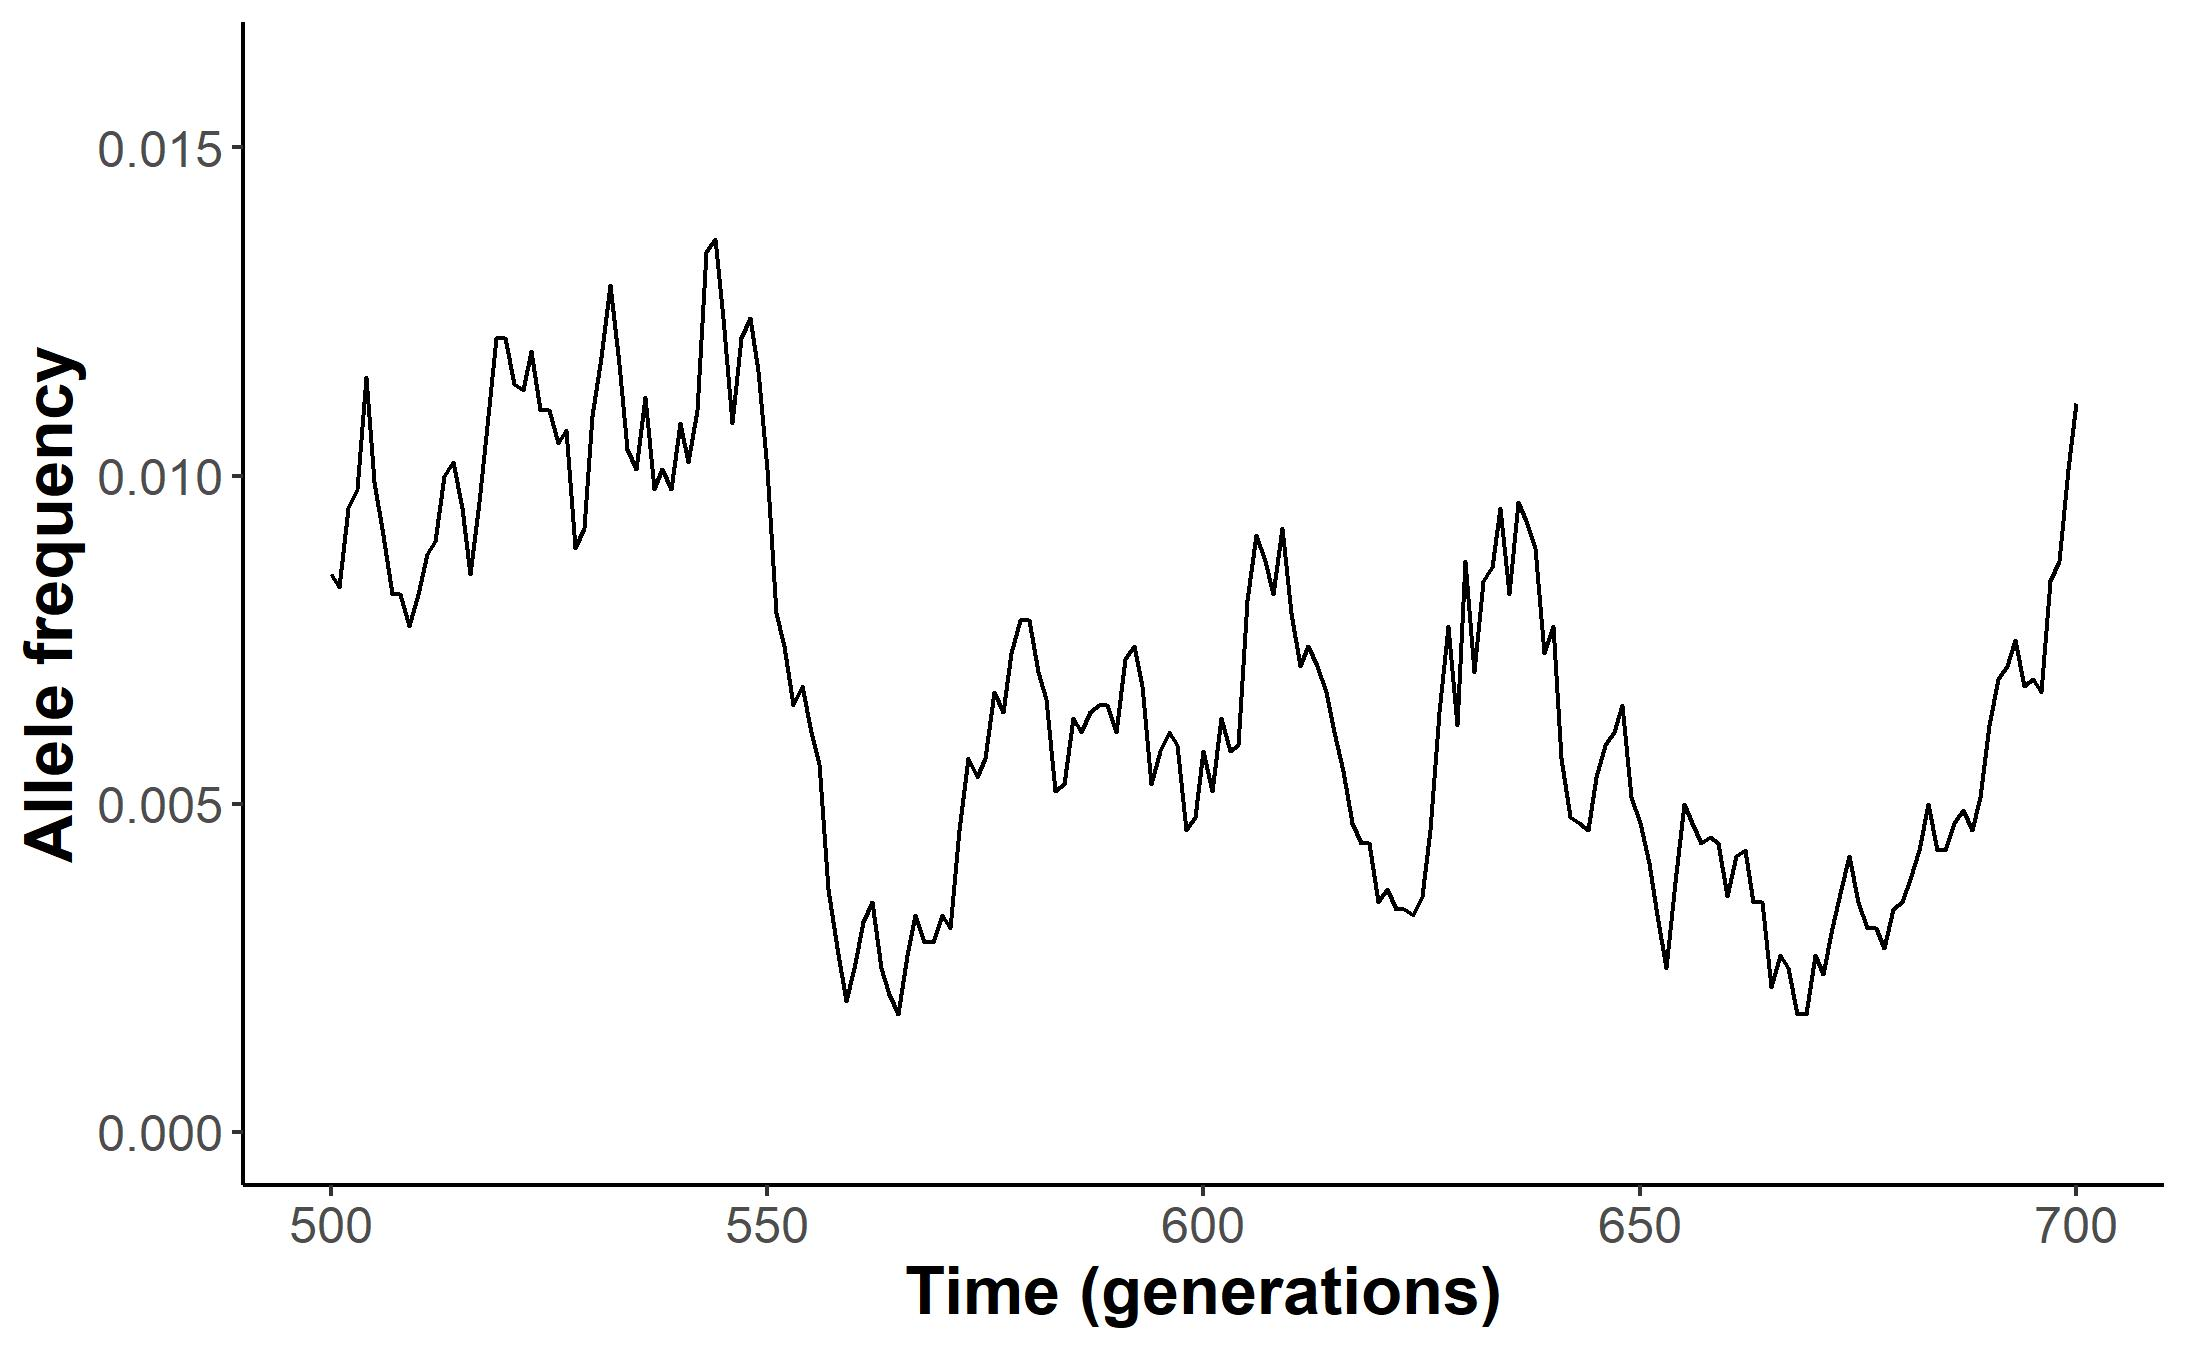
\includegraphics[scale=0.5]{img/time_series.jpg}
    \caption{An example simulation output plot of allele frequencies changing over time.}
    \label{fig:time_series}
\end{figure}

\subsubsection{SLiM}

Here we describe our use of \code{SLiM} to generate simulations of our model. \code{SLiM} operates with its own scripting language called \code{Eidos} (named after the Platonic forms). This language provides an interface to \code{SLiM} functionality that is flexible, albeit sometimes challenging to work with. The main difficulty with \code{SLiM} is that it requires each evolutionary process to essentially be defined separately from one another. As opposed to writing a single line of code to capture all evolutionary forced of interest, \code{SLiM} requires individual function calls for specifying rates of mutation, migration, selection, etc. Additionally, blocks of code are performed according to the generation time specified. The general schematic is shown:


\lstinputlisting[language=Eidos, caption = SLiM simulation script skeleton]{src/slim_skeleton.txt}

An \code{initialize()\{\}} block defines properties of the genomes to simulate (diploid genomes by default). This is executed before the simulation begins to run. Spatial population parameters can be specified at the first generation of the simulation, in the \code{1\{\}} block. Finally, the \code{20000 late()\{\}} block specifies how long to run the simulation for, and what to do at the end of the simulation. We show the script used to simulate the Stepping Stone migration model with expanded Wright-Fisher dynamics (migration, mutation, selection, and genetic drift included). The script reads population parameters from \code{Python} file defined similarly to listing \ref{code:params}. 

\lstinputlisting[language=Eidos, caption = SLiM script used to simulate Wright-Fisher + Stepping Stone model]{src/slim_2d_ss.txt}


Clearly, \code{SLiM} code becomes unnecessarily complex for a model that ought to be written in a single line of code. We used \code{SLiM} for our early experimentation, but quickly moved towards writing our own programs once we realized that we don't need much of the added \code{SLiM} functionality. The next section explores our custom-built simulations. The remaining data presented in this paper will use results collected from these \code{Python} simulations.

\subsubsection{NumPy}

As mentioned, \code{NumPy} allows us to efficiently run simulations of our model. We can define a \code{SS\_WF\_sim()} function to accept our population parameters and calculate $df$ given by equation (\ref{eq:model}). We perform this calculation for every generation, storing a matrix $\bf{f}$ containing allele frequencies over time at each deme. Stochasticity is incorporated into our population using \code{NumPy} random number generators. We store these matrices as \code{.npy} \textit{byte} files which save on storage space and allow other \code{NumPy} programs to quickly load in our data. The script used to perform our simulations is shown below:

\lstinputlisting[language=iPython, caption = Python script used to simulate Wright-Fisher + Stepping Stone model]{src/python_ss_wf.py}

This script is much more concise than our \code{SLiM} script and offers computation speed that is orders of magnitude faster. We use \code{np.random.binomial()} to generate binomial random samples given probability $p = f_{t-1} + df$. This simulates genetic drift through the manner described in section  \ref{section:neutral_wf}. What may be less clear is our use of \code{laplace()} from the \code{SciPy} package \cite{scipy} to incorporate migration. In mathematical terms, the \code{laplace()} function computes the \textit{Laplacian} of our frequency matrix $\textbf{f}$ and performs a \text{convolution} of our matrix with its Laplacian. The Laplacian of a function $\psi$ (written $\nabla^2 \psi$) is defined as the following:

\begin{equation}
    \nabla^2 \psi(x,y) =  \frac{\partial^2 f}{\partial x^2} + \frac{\partial^2 f}{\partial y^2}
\end{equation}

Essentially, the Laplacian is a sum of all of the unmixed second partial derivatives of $\psi$. What does this have to do with migration? It turns out that there is another way to write the form of the Laplacian:

\begin{equation}
    \nabla^2 \psi(x,y) =  \frac{1}{h^2}(\psi_{x+h,y} + \psi_{x-h,y} + \psi_{x,y+h} + \psi_{x,y-h} - 4\psi_{x,y})
\end{equation}

When we set $h = 1$, $\psi(x,y) = \frac{df}{dt}(r,s)$ and multiply by migration rate $m$, we arrive at our equation for migration dynamics in the two-dimensional Stepping Stone model:

\begin{equation} 
    \tag{\ref{eq:stepstone} revisited}
    m[\nabla^2 df_{r,s}] = m(f_{r-1,s} + f_{r+1,s} + f_{r,s+1} + f_{r,s-1} - 4f_{r,s})dt
\end{equation}


The \code{laplace()} generalizes our simulation to as many spatial dimensions as specified in the \code{dims} parameter. We use the exact same script to simulate Stepping Stone migration in both one and two dimensional models. When we call the \code{laplace()} function on our matrix $\text{bf}$, the calculation in equation \ref{eq:stepstone} is performed across all pairs of $(r,s)$ neighbor demes and $df$ is computed accordingly. All this is done in a computationally efficient, generalized fashion.


We perform many replicate simulations over various combinations of population parameters. Because our simulations are stochastic, we need many replicates to compute useful statistics and relate our theoretical predictions to our generated data. Our goal is essentially to explore how changing the aforementioned population parameters influences what we see in our simulations. To demonstrate how altering some parameters changes the dynamics of our model, we present a collection of simulated allele frequency trajectories in a one-deme, neutral Wright-Fisher model ($\mu = s = m = 0$). We vary the population size $N$ and the initial allele frequency $f_0$ and observe changes due to genetic drift. Recall the following properties:

\begin{equation}
    \tag{\ref{eq:ex_drift} revisited}
    E[f_t] = f_0
\end{equation}

\begin{equation}
    \tag{\ref{eq:var_lim_drift} revisited}
    \lim_{N \to \infty} Var[f_{t+1}] = 0
\end{equation}


Figure (\ref{fig:neutral_wf}) neatly demonstrates these properties while also illustrating the time dynamics of the neutral Wright-Fisher model. 


\begin{figure}[h]
    \centering
    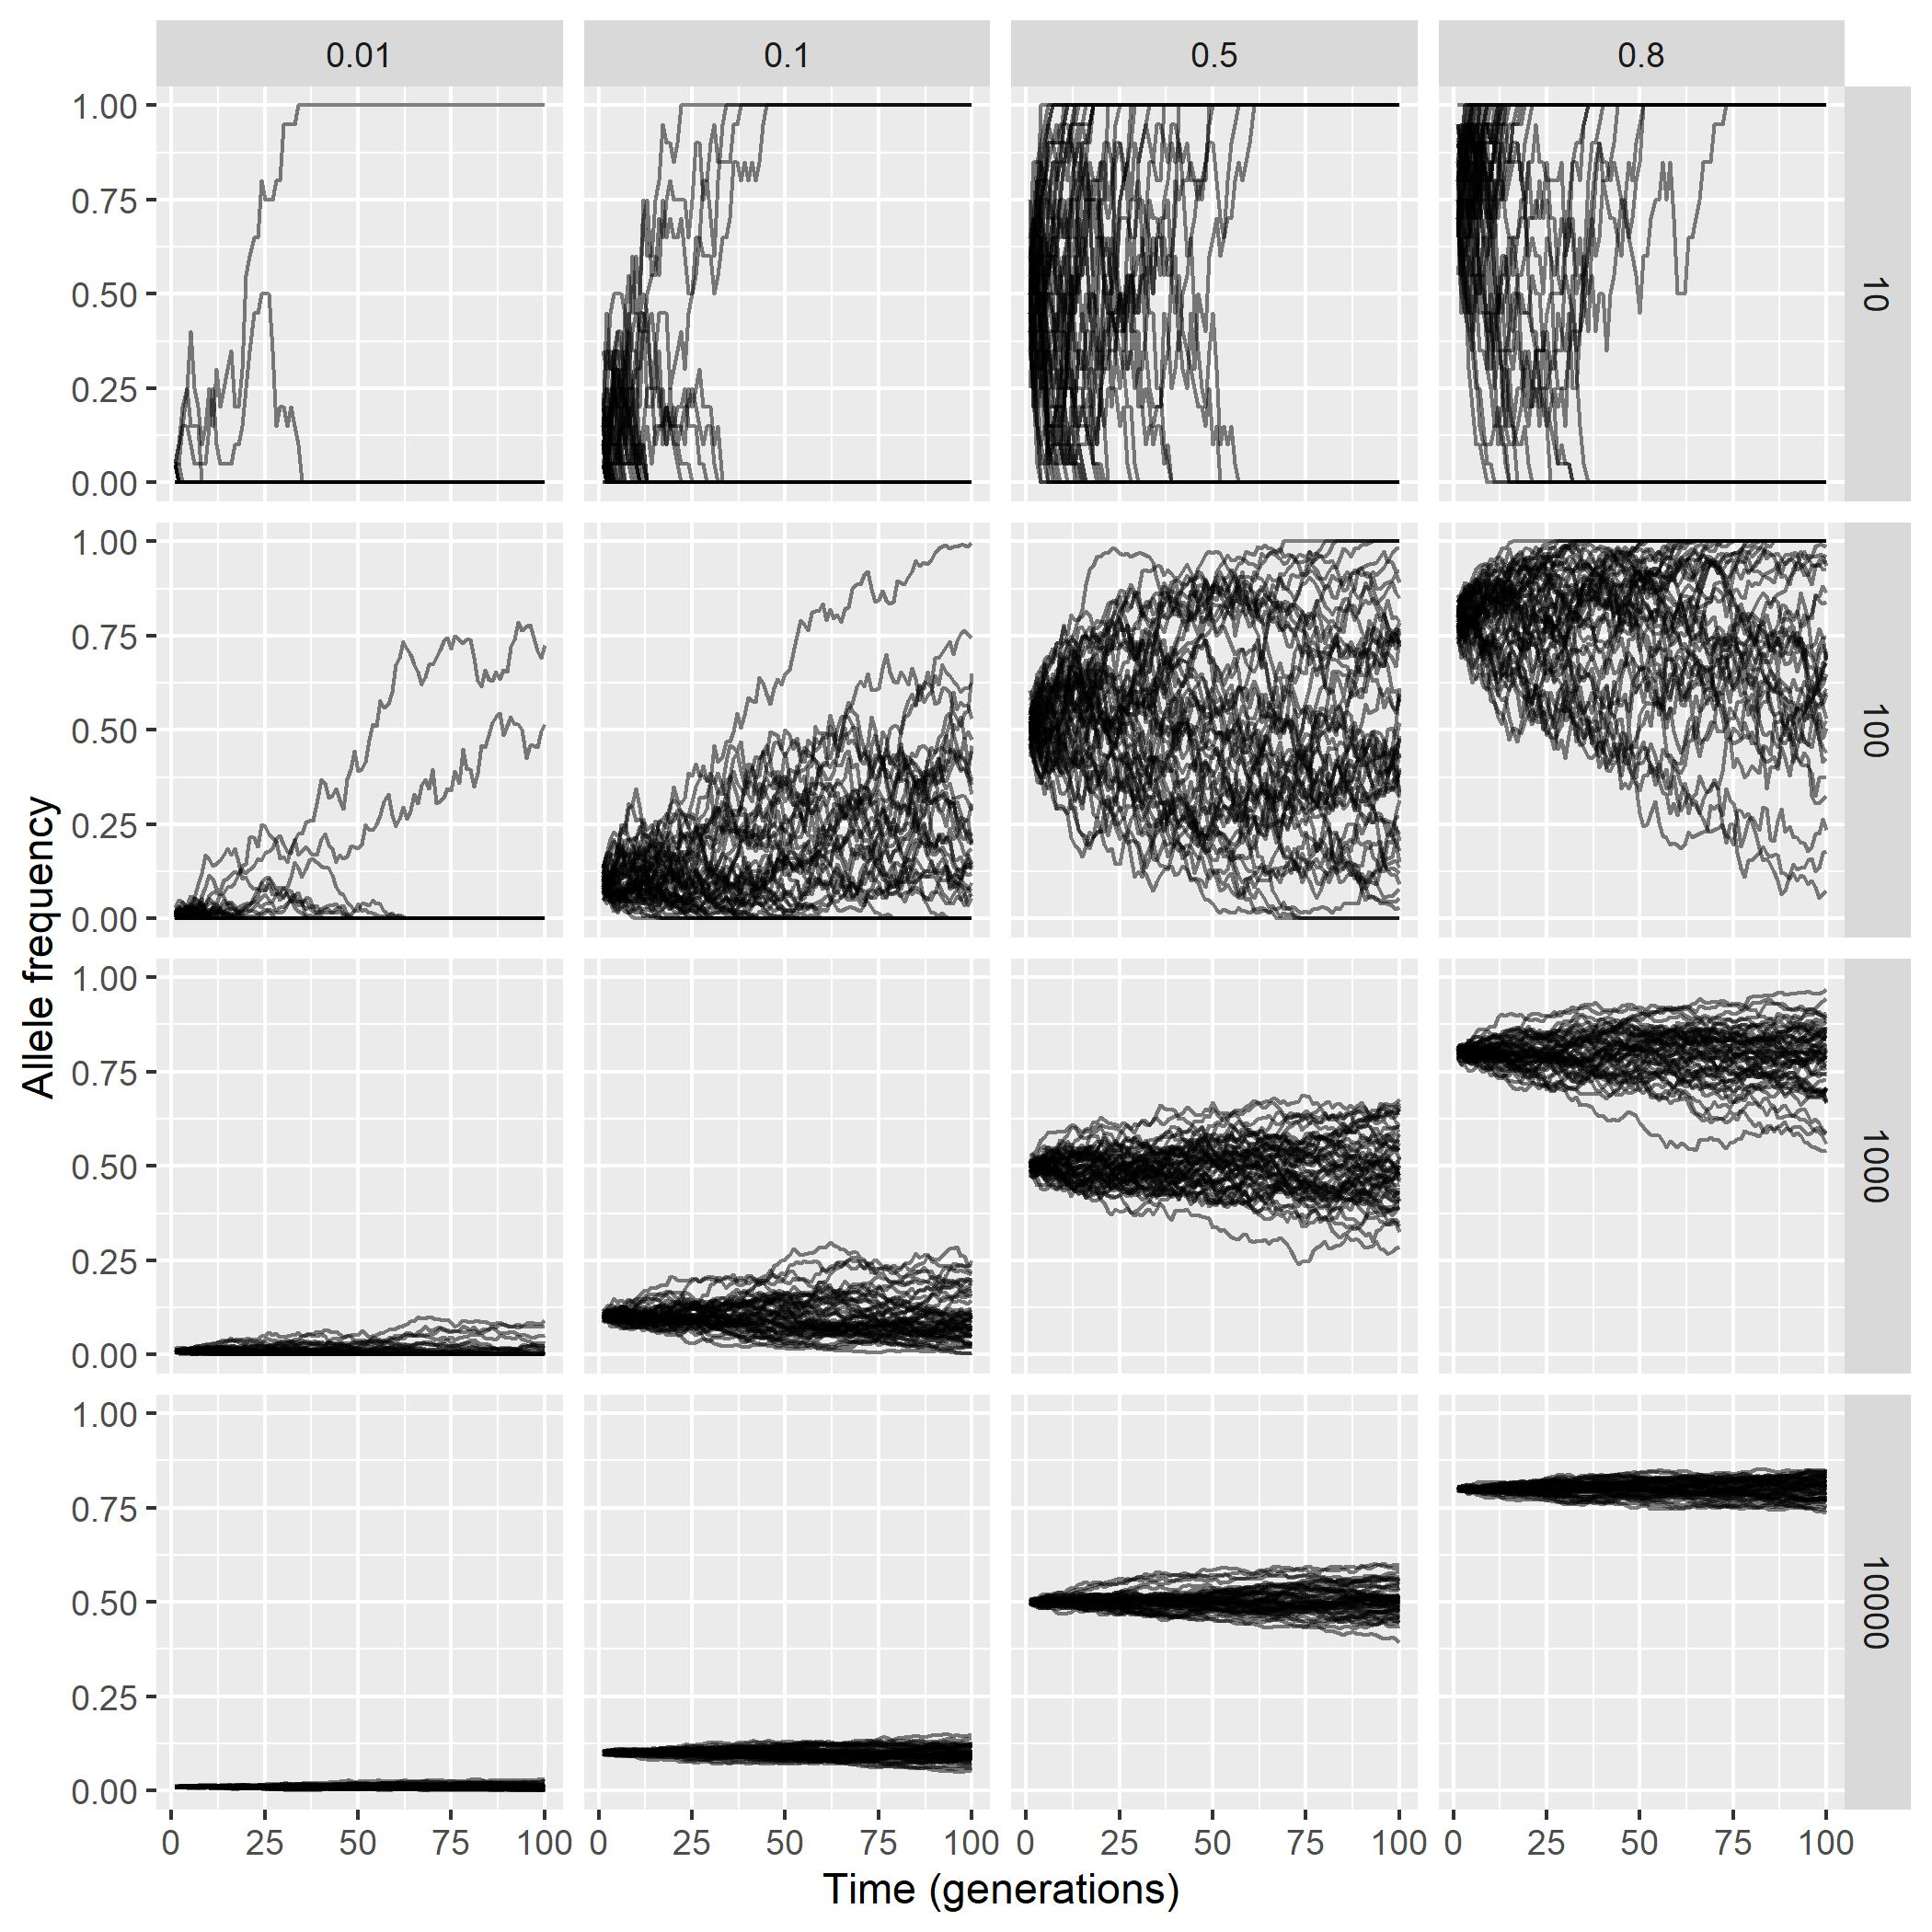
\includegraphics[scale=0.8]{img/neutral_wf.jpg}
    \caption{This figure shows several simulated trajectories for varying initial allele frequency $f_0$ and population size $N$ in a one deme, neutral Wright-Fisher model. Each row shows simulations run with a common $N$ and each column shows a common $f_0$. Figure formatting is inspired by Novembre lab member Joe Marcus' \textit{Introduction to the Wright-Fisher model}.\cite{marcus_2016}}
    \label{fig:neutral_wf}
\end{figure}




\newpage
\subsection{Simulated sampling}
This section describes our method for simulating the sampling process inherent in GWAS. Recall that we are interested in the interaction between the underlying distribution of allele frequencies and the distribution of frequencies observed in a population sample (Figure: \ref{fig:sampling_schematic}). We expect the ability to detect alleles in a GWAS sample to depend on the population parameters (particularly the rates of selection and migration) and on the strategy used to select members of a GWAS corhort. Geography plays a key role in the search of rare disease-causing alleles. Intuitively, \texit{where} researchers sample individuals from and \textit{how many} individuals are sampled from each location determines which alleles are detectable.


Essentially, we want to randomly draw alleles from our simulated population according to some sampling probability distribution. We accomplish this by computing a \textit{convolution} with our allele frequency matrix $\textbf{f}$. A convolution of discrete-valued functions $f$ and $g$ is defined as:

\begin{equation}\label{eq:convolution}
    (f*g)(r) = \sum_{d=-\infty}^\infty f(r)g(r-d)
\end{equation}


Where $f$ and $g$ are both functions of $r$, the convolution expresses how $g$ changes the shape of $f$ over all $g(r)$. For our model, we assume a Gaussian sampling distribution centered at a deme $\hat{r}$ with a specified standard deviation, or width, $w$. The convolution allows us to compute the average probability of sampling the allele over all possible centers $\hat{r}$. The output of this calculation is another matrix of sampled allele frequencies $\bf{F}$ that is of the same dimensions as $\bf{f}$. The following code snippet shows our implementation of this process using the \code{SciPy} Gaussian convolution filter. 


\lstinputlisting[language=iPython, caption = Python script to implement sampling process]{src/sample.py}


We can now add $w$ to our list of simulation parameters. Our results primarily focus on exploring the relationships between our population parameters. Altering our parameters changes the allele frequency trajectories observed, providing insight into how the evolutionary process and the sampling process influence allele detection.        


%% End with mentioning Snakemake?

\chapter{Results}
\section{Important Quantities from Our Model}
As shown in the previous chapter, our model describes the change in allele frequencies over time and space. Evolutionary forces act to shape the distribution of alleles across our simulated geographic habitat. There are two immediate questions that we will utilize our model to answer:

\begin{enumerate}
    \item How much of the allele do we expect to observe?
    \item Where can we expect to find the allele?
\end{enumerate}


For a more intuitive understanding of what each of these questions represent, let us examine the raw simulation output from our model. We simulate a single genetic locus and record the frequency of the minor, or \textit{focal} allele $f(a)$ after thousands of simulated generations. Allele frequencies vary across geographic position, but tend to be higher in some neighboring demes. This represents the localization of rare alleles observed in natural populations. \cite{1000_genomes} \cite{geerlings_2018} \cite{novembre_marcus_2017} 


\begin{figure}[h]
    \centering
    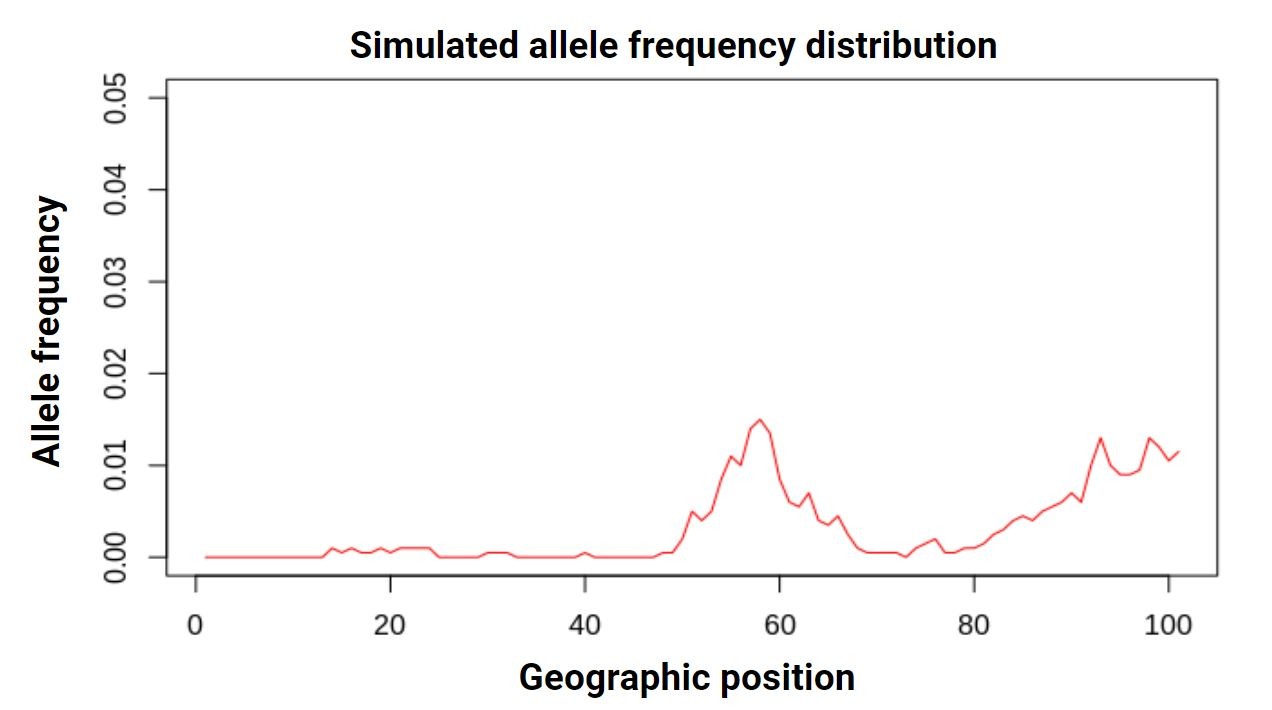
\includegraphics[scale=0.4]{img/geographic_distribution.JPG}
    \caption{The geographic distribution of the focal allele in a single simulation with a single set of evolutionary parameters ($\mu,s,m,N$). We allow for thousands of generations of time to pass to allow our simulation to approach equilibrium.}
    \label{fig:geog_sim}
\end{figure}


We observe a peak in the simulated example (Figure: \ref{fig:geog_sim}) that illustrates the geographic range of the allele. New alleles come into existence at one particular location. Some of these will reach higher frequencies in the population and some will spread farther beyond their initial position. The height of these peaks tells us how much of the allele we can expect to observe, and the width of these peaks tells us where we can expect to observe it. It is clear that alleles that reach, on average, higher frequencies will be easier to observe. We will calculate the average allele frequency and the geographic range of an allele to answer our initial questions.



\subsection{The average allele frequency}


 

\subsection{The geographic range of the allele}


\section{Computing the Expected Site Frequency Spectrum}

\section{Measuring Missing Heritability}

% Format a LaTeX bibliography
\makebibliography
%\bibliography{references}

% Figures and tables, if you decide to leave them to the end
%\input{figure}
%\input{table}

\end{document}


